\documentclass[12pt]{article}
\usepackage[margin=1in]{geometry}
\usepackage{setspace}
\usepackage{array}
\usepackage{enumitem}
\usepackage{titlesec}
\usepackage{graphicx}
\usepackage{microtype}
\usepackage[dvipsnames]{xcolor}
\usepackage[hidelinks]{hyperref}
\usepackage{url}

\setlength{\parindent}{0pt}
\setlength{\parskip}{6pt}
\setlength{\emergencystretch}{2em}
\setstretch{1.12}
\urlstyle{same}

\titleformat{\section}
  {\Large\bfseries\color{MidnightBlue}}
  {\thesection}{0.6em}{}
\titleformat{\subsection}
  {\large\bfseries\color{NavyBlue}}
  {\thesubsection}{0.6em}{}

\begin{document}

% -------------------- COVER PAGE --------------------
\begin{titlepage}
\centering

\vspace*{1cm}
{\large Course Project Writeup}

\vspace{4cm}

{\Huge \textbf{Pokemon OOP Explorer}}

\vspace{0.5cm}
\rule{0.8\textwidth}{0.5pt}

\vspace{0.5cm}
{\large \url{https://github.com/avih7531/pokemon-oop-explorer}}

\vspace{3cm}

\vspace{0.5cm}
Avi Herman (AJH773)

\vfill

\begin{flushleft}
Date of Submission: \today
\end{flushleft}

\end{titlepage}

% -------------------- TABLE OF WORK --------------------
\newpage
\begin{center}
{\LARGE \textbf{Table of Work}} \\[0.5em]
{\small (Please write x in the boxes to mention what each student achieved in this project)}
\end{center}

\vspace{1cm}

\renewcommand{\arraystretch}{1.8}
\begin{tabular}{|p{6cm}|c|c|c|}
\hline
 & Avi & Student-2 & Student-3 \\
\hline
Project Description & x &  &  \\
\hline
Uses Cases Diagram(s) and discription & x &  &  \\
\hline
Sequence Diagrams & x &  &  \\
\hline
Class diagram(s) & x &  &  \\
\hline
Implementation & x &  &  \\
\hline
Conclusion & x &  &  \\
\hline
\end{tabular}

% -------------------- TABLE OF CONTENTS --------------------
\newpage
\begin{center}
{\LARGE \textbf{Table of Contents}}
\end{center}

\vspace{1cm}

\begin{itemize}[leftmargin=1.5cm]

\item System Analysis
    \begin{itemize}
        \item Written Project description (One Page)
            \begin{itemize}
                \item General Description, Goals and Benefits
                \item Special requirements (Performance, Interfaces, Constraints, Reliability, if any)
            \end{itemize}
        \item Uses Cases Diagram(s) and use cases description.
    \end{itemize}

\item System Design
    \begin{itemize}
        \item Sequence Diagrams
        \item Class diagram(s)
    \end{itemize}

\item Conclusion (work summary, difficulties, recommendations, ..)

\item Appendix (any related reports, questionnaires, docs..)

\end{itemize}

% -------------------- REPORT CONTENT --------------------
\newpage
\section*{System Analysis}

\begin{center}
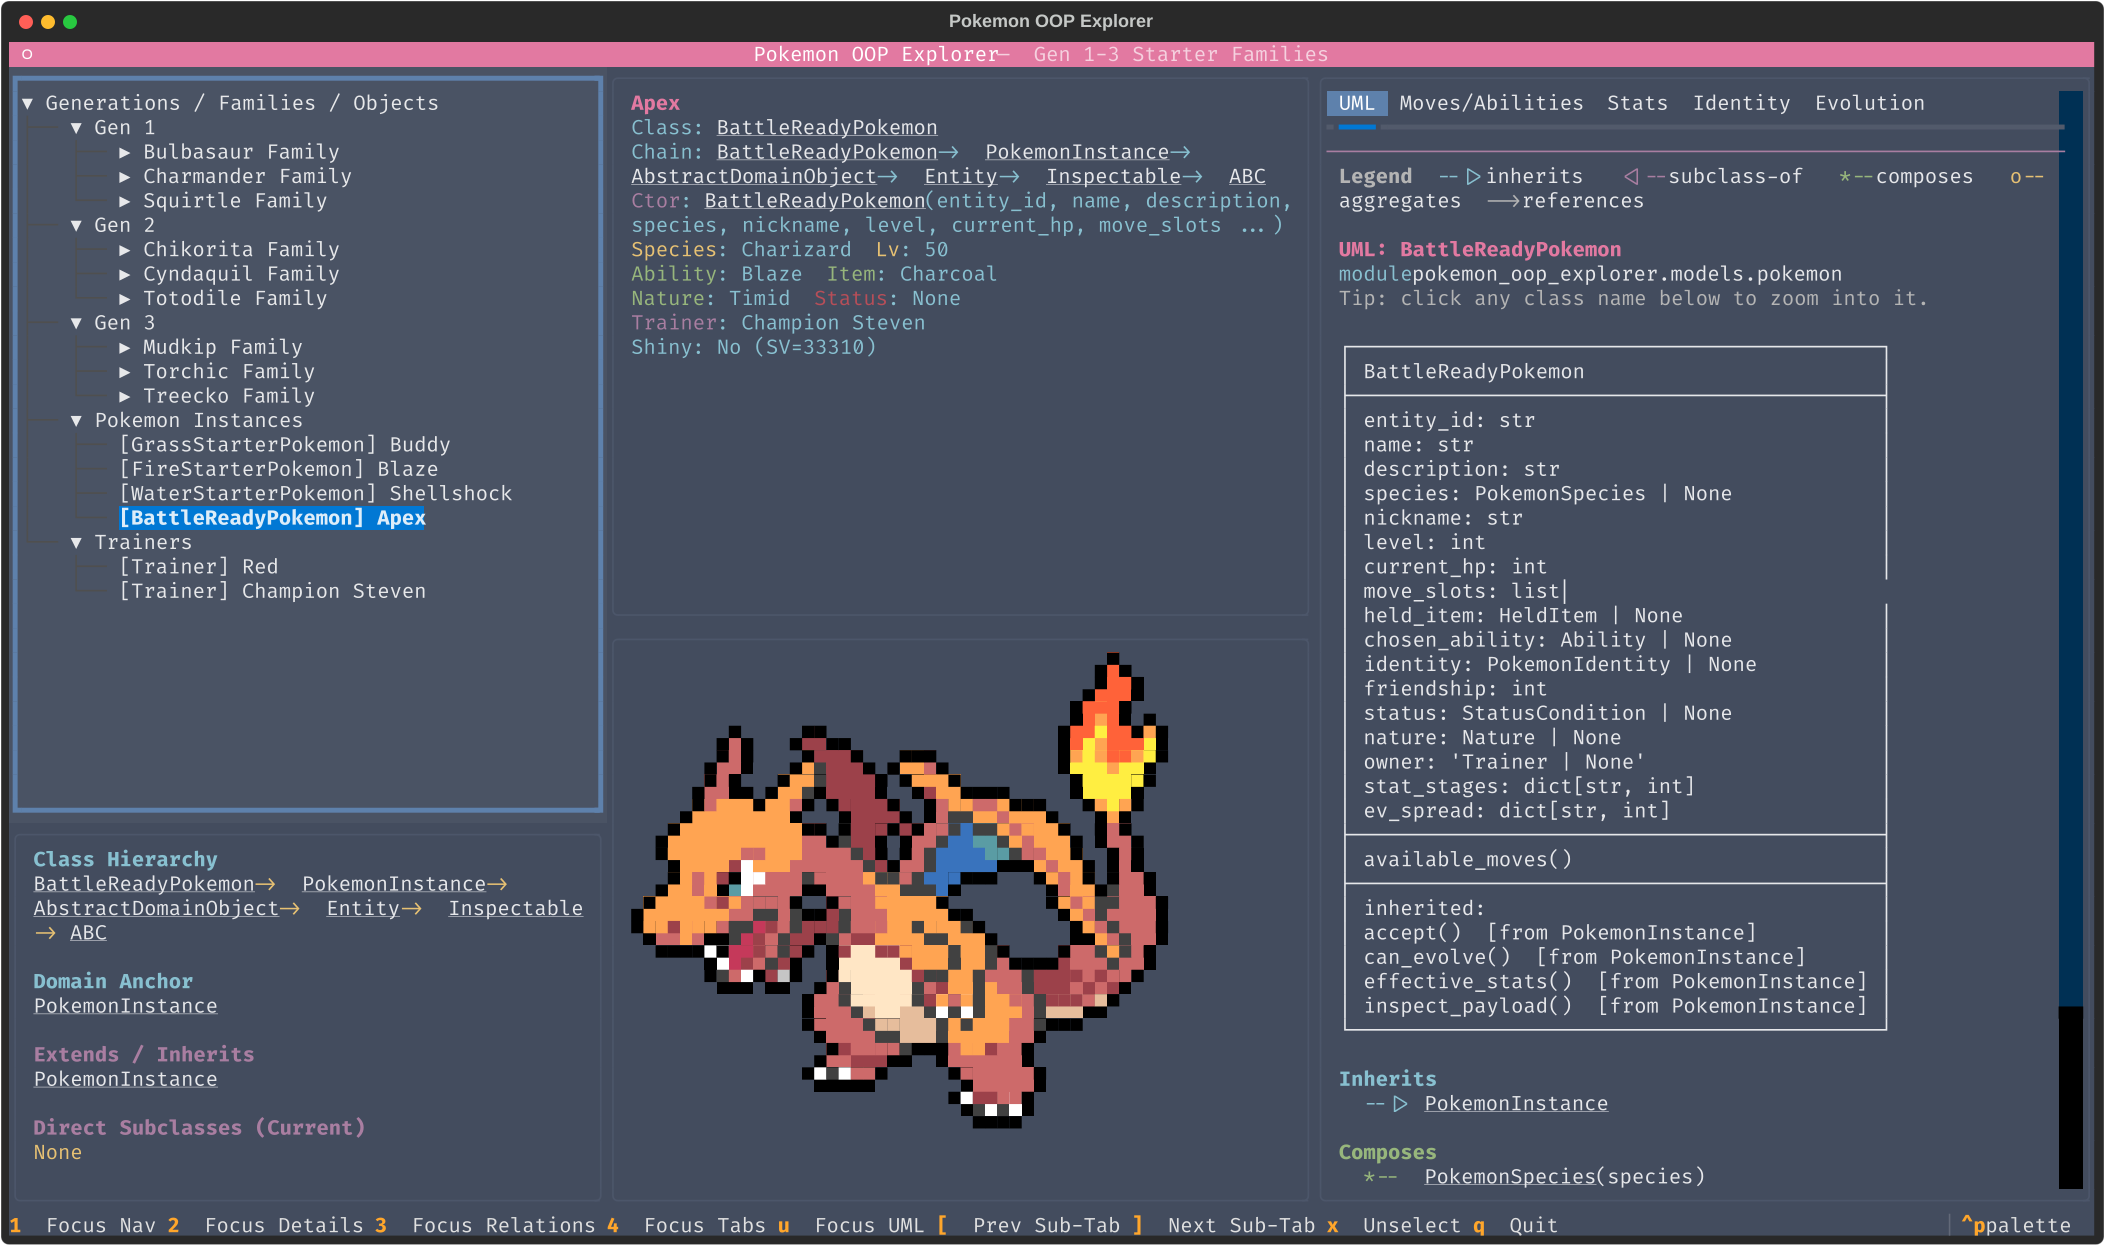
\includegraphics[width=\textwidth,keepaspectratio]{../image.png}
\end{center}
\textit{Figure: Application preview.}

\subsection*{Written Project Description}
\textbf{General Description}\\
Pokemon OOP Explorer is a terminal-based software system built to explore a
well-scoped Pokemon domain model for Gen 1--3 starter families. Instead of
focusing on a complete Pokedex or competitive battle simulator, this project
focuses on object-oriented software engineering concepts: inheritance,
composition, polymorphism, abstract interfaces, and clean separation of
responsibilities. The application is implemented with Textual (TUI) and is
organized in modular layers: models, services, introspection utilities, and UI
presentation.

\textbf{Goals and Benefits}\\
The project goals are:
\begin{itemize}
    \item Build a clear and maintainable object-oriented domain with
    behavior-rich classes, not just passive data structs.
    \item Provide an interactive inspector where users can navigate species,
    instances, and trainers, and inspect relationships in real time.
    \item Demonstrate important OOP patterns in practice: Visitor, Strategy
    (for graph edge detection), and Composite (for evolution rules).
    \item Produce UML artifacts that reflect the real implementation so design
    and code stay aligned.
\end{itemize}

The main benefits are educational and structural: the system makes OOP design
decisions visible, testable, and reviewable, while keeping the domain scope
small enough to reason about deeply.

\textbf{Special Requirements}\\
\begin{itemize}
    \item \textbf{Performance:} The app runs locally on seeded/cached data and
    avoids live API dependency during normal usage, which keeps interactions
    responsive.
    \item \textbf{Interface constraints:} The UI requires a large terminal
    footprint for proper three-pane rendering and Unicode/ANSI compatibility.
    \item \textbf{Reliability:} Domain behavior is covered by automated tests
    (repository, evolution logic, identity, effects, class graph, and trainer
    operations), improving confidence in correctness.
    \item \textbf{Scope constraints:} Limited intentionally to Gen 1--3
    starter lines and related trainer/instance identity/evolution flows.
\end{itemize}

\subsection*{Use Cases Diagram(s) and Use Case Description}
The actor is a student/reviewer exploring and evaluating the domain model.
Use-case and activity UML diagrams are provided under:
\begin{itemize}
    \item \url{docs/uml/use_cases/images/overview.png}
    \item \url{docs/uml/use_cases/images/uc-1_...png} through
    \url{uc-8_...png}
\end{itemize}

The implemented use cases are:
\begin{itemize}
    \item UC-1 Browse catalog
    \item UC-2 Inspect domain objects
    \item UC-3 View class relationships
    \item UC-4 Review moves and abilities
    \item UC-5 Analyze stats
    \item UC-6 Explore identity mechanics
    \item UC-7 Trace evolution
    \item UC-8 Preview sprites
\end{itemize}

\textbf{Use Case Description Tables (Reference Format)}\\
\textit{Primary actor for all use cases: Student/Reviewer using the terminal
application.}

\subsubsection*{UC-1 Browse catalog}
\begin{tabular}{|p{0.30\textwidth}|p{0.62\textwidth}|}
\hline
\textbf{UC Reference Name/Number} & \textbf{UC-1 Browse catalog} \\
\hline
\textbf{Overview} & Open the app and navigate the tree by generation, family,
and object type to locate species, instances, and trainers for inspection. \\
\hline
\textbf{Related use cases} & UC-2, UC-3, UC-4, UC-5, UC-6, UC-7, UC-8 \\
\hline
\textbf{Actors} & Student/Reviewer \\
\hline
\end{tabular}

\subsubsection*{UC-2 Inspect domain objects}
\begin{tabular}{|p{0.30\textwidth}|p{0.62\textwidth}|}
\hline
\textbf{UC Reference Name/Number} & \textbf{UC-2 Inspect domain objects} \\
\hline
\textbf{Overview} & Select a domain object and review structured payload data
including class context, typed fields, and object-specific details. \\
\hline
\textbf{Related use cases} & UC-1, UC-3, UC-4, UC-5, UC-6, UC-7, UC-8 \\
\hline
\textbf{Actors} & Student/Reviewer \\
\hline
\end{tabular}

\subsubsection*{UC-3 View class relationships}
\begin{tabular}{|p{0.30\textwidth}|p{0.62\textwidth}|}
\hline
\textbf{UC Reference Name/Number} & \textbf{UC-3 View class relationships} \\
\hline
\textbf{Overview} & View inheritance and composition/aggregation links for the
selected class using the relationship panel and UML-focused rendering. \\
\hline
\textbf{Related use cases} & UC-1, UC-2, UC-4, UC-5, UC-6, UC-7 \\
\hline
\textbf{Actors} & Student/Reviewer \\
\hline
\end{tabular}

\subsubsection*{UC-4 Review moves and abilities}
\begin{tabular}{|p{0.30\textwidth}|p{0.62\textwidth}|}
\hline
\textbf{UC Reference Name/Number} & \textbf{UC-4 Review moves and abilities} \\
\hline
\textbf{Overview} & Open the Moves/Abilities tab to inspect learnsets, move
slots, categories, and ability assignments for species and instances. \\
\hline
\textbf{Related use cases} & UC-1, UC-2, UC-5 \\
\hline
\textbf{Actors} & Student/Reviewer \\
\hline
\end{tabular}

\subsubsection*{UC-5 Analyze stats}
\begin{tabular}{|p{0.30\textwidth}|p{0.62\textwidth}|}
\hline
\textbf{UC Reference Name/Number} & \textbf{UC-5 Analyze stats} \\
\hline
\textbf{Overview} & Open the Stats tab to inspect base stats and effective
stat outputs after nature and status condition effects are applied. \\
\hline
\textbf{Related use cases} & UC-1, UC-2, UC-4, UC-6, UC-7 \\
\hline
\textbf{Actors} & Student/Reviewer \\
\hline
\end{tabular}

\subsubsection*{UC-6 Explore identity mechanics}
\begin{tabular}{|p{0.30\textwidth}|p{0.62\textwidth}|}
\hline
\textbf{UC Reference Name/Number} & \textbf{UC-6 Explore identity mechanics} \\
\hline
\textbf{Overview} & Open the Identity tab to inspect identity labels and
Gen-3-style shiny computation fields tied to each Pokemon instance. \\
\hline
\textbf{Related use cases} & UC-1, UC-2, UC-5, UC-8 \\
\hline
\textbf{Actors} & Student/Reviewer \\
\hline
\end{tabular}

\subsubsection*{UC-7 Trace evolution}
\begin{tabular}{|p{0.30\textwidth}|p{0.62\textwidth}|}
\hline
\textbf{UC Reference Name/Number} & \textbf{UC-7 Trace evolution} \\
\hline
\textbf{Overview} & Open the Evolution tab to inspect evolution lines and
evaluate rule-based evolution eligibility using context-aware constraints. \\
\hline
\textbf{Related use cases} & UC-1, UC-2, UC-3, UC-5 \\
\hline
\textbf{Actors} & Student/Reviewer \\
\hline
\end{tabular}

\subsubsection*{UC-8 Preview sprites}
\begin{tabular}{|p{0.30\textwidth}|p{0.62\textwidth}|}
\hline
\textbf{UC Reference Name/Number} & \textbf{UC-8 Preview sprites} \\
\hline
\textbf{Overview} & Display regular/shiny sprite output from local assets for
selected instances, with fallback behavior when a sprite is unavailable. \\
\hline
\textbf{Related use cases} & UC-1, UC-2, UC-6 \\
\hline
\textbf{Actors} & Student/Reviewer \\
\hline
\end{tabular}

\newpage
\section*{System Design}

\subsection*{Sequence Diagrams}
Sequence diagrams are included for the main runtime interactions and logic
paths, with method names aligned to implementation code:
\begin{itemize}
    \item \url{full_sequence_diagram.png}
    \item \url{seq_1_app_startup.png}
    \item \url{seq_2_node_selection_refresh.png}
    \item \url{seq_3_zoom_class.png}
    \item \url{seq_4_evolution_check.png}
    \item \url{seq_5_trainer_party_update.png}
    \item \url{seq_6_identity_mechanics.png}
    \item \url{seq_7_stats_analysis.png}
\end{itemize}

These sequences cover startup, selection rendering, UML focusing, evolution
rule evaluation, trainer-party ownership updates, identity/shiny inspection,
effective stat computation, and a full end-to-end interaction timeline.

\subsection*{Class Diagram(s)}
The class diagram is provided in:
\begin{itemize}
    \item \url{docs/uml/class_diagram/images/full_class_diagram.png}
    \item \url{docs/uml/class_diagram/images/domain_class_diagram.png}
\end{itemize}

It models:
\begin{itemize}
    \item Core contracts (\texttt{Inspectable}, \texttt{AbstractDomainObject},
    \texttt{Evolvable})
    \item Pokemon domain entities (\texttt{PokemonSpecies},
    \texttt{PokemonInstance}, \texttt{Trainer})
    \item Evolution hierarchy (\texttt{EvolutionRule} and concrete rule types)
    \item Visitor components (\texttt{DomainVisitor},
    \texttt{ClassUsageVisitor}, \texttt{SummaryVisitor})
    \item Application and services (\texttt{PokemonExplorerApp},
    \texttt{DomainRepository}, \texttt{SpriteService}, graph builder/renderer)
\end{itemize}

Key required methods are explicitly represented as implemented:
\texttt{accept}, \texttt{inspect\_payload}, \texttt{can\_evolve},
\texttt{effective\_stats}, and \texttt{add\_to\_party}.

\section*{Conclusion}
This project successfully demonstrates a focused OOP system with clear design
boundaries and traceable UML documentation. The strongest outcomes are:
\begin{itemize}
    \item A behavior-rich object model rather than a purely data-centric model.
    \item Practical use of OOP design patterns in a real codebase.
    \item Consistency between implementation and UML artifacts.
    \item Test-backed reliability for key domain mechanics.
\end{itemize}

Difficulties included balancing diagram completeness with scope, keeping
sequence messages aligned with real method calls, and maintaining visual
consistency across all UML outputs. Recommended next steps would be extending
the same architecture to additional Pokemon families and adding more
interaction-level tests for UI workflows.

\section*{Appendix}
\textbf{Artifact locations}
\begin{itemize}
    \item Use-case diagrams: \url{docs/uml/use_cases/}
    \item Class diagram: \url{docs/uml/class_diagram/}
    \item Sequence diagrams: \url{docs/uml/sequences/}
    \item Source code root: \url{pokemon_oop_explorer/}
\end{itemize}

\textbf{Diagram viewing note:} Most UML diagrams are intentionally dense.
Please zoom in when viewing this PDF. You can also open each image directly in
its source folder under \texttt{docs/uml/}.

\textbf{Coverage note:} The codebase contains \textbf{194} defined
functions/methods in \texttt{pokemon\_oop\_explorer/}. Using all UML source
files in \texttt{docs/uml/**/*.puml}, \textbf{81} definitions are represented
explicitly and \textbf{113} are not explicitly represented. This is intentional:
the diagrams emphasize architecture-critical behavior rather than every helper.

\newpage
\section*{UML Diagram Gallery}

\subsection*{Use Cases}
\textit{Zoom recommended for these diagrams. Source folder:
\texttt{docs/uml/use\_cases/images/}.}

\begin{center}
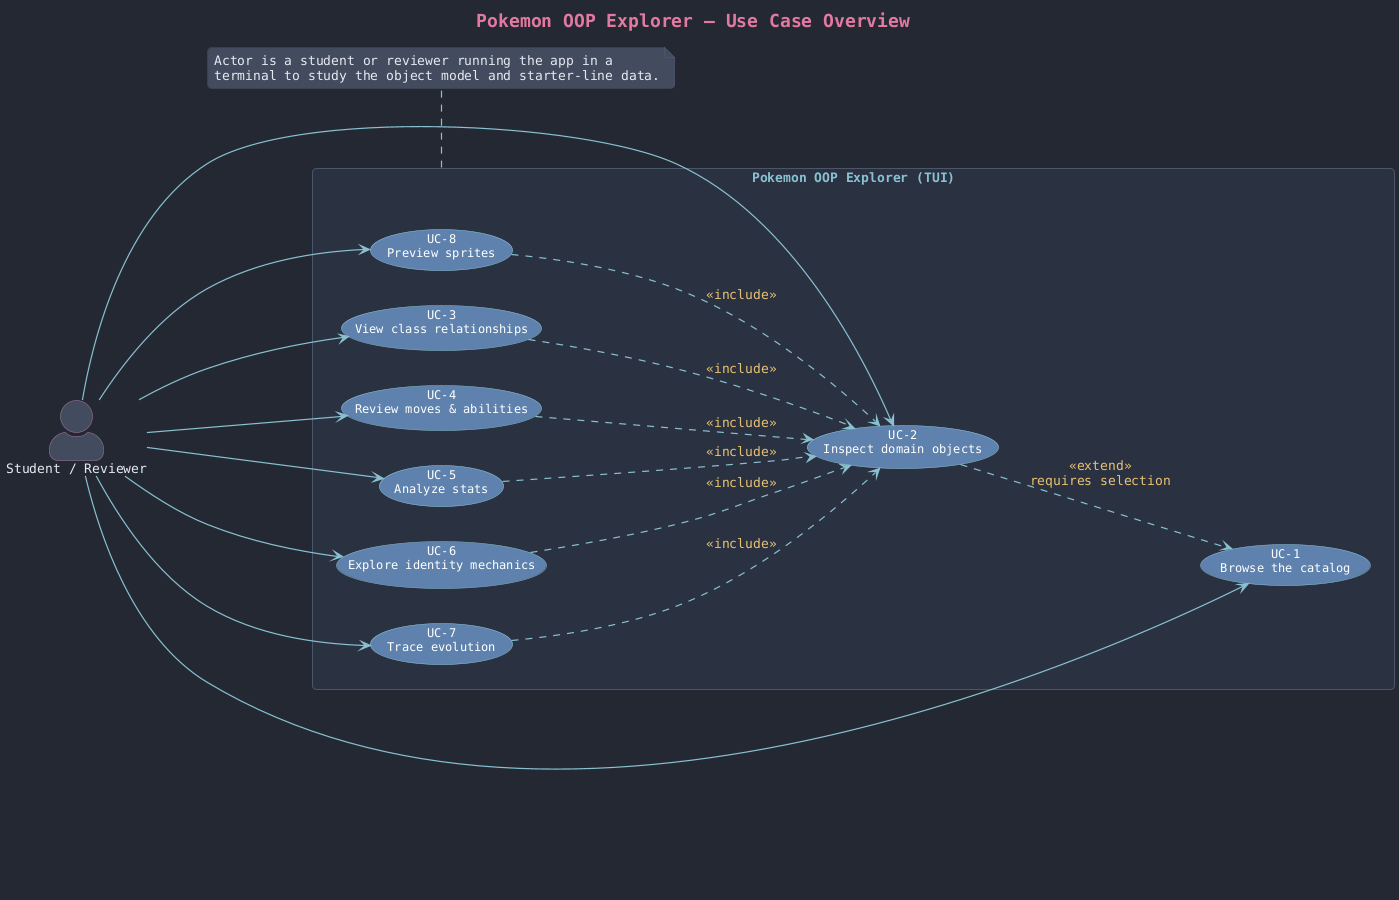
\includegraphics[width=\textwidth,keepaspectratio]{../docs/uml/use_cases/images/overview.png}
\end{center}
\textit{Overview use-case diagram.}

\begin{center}
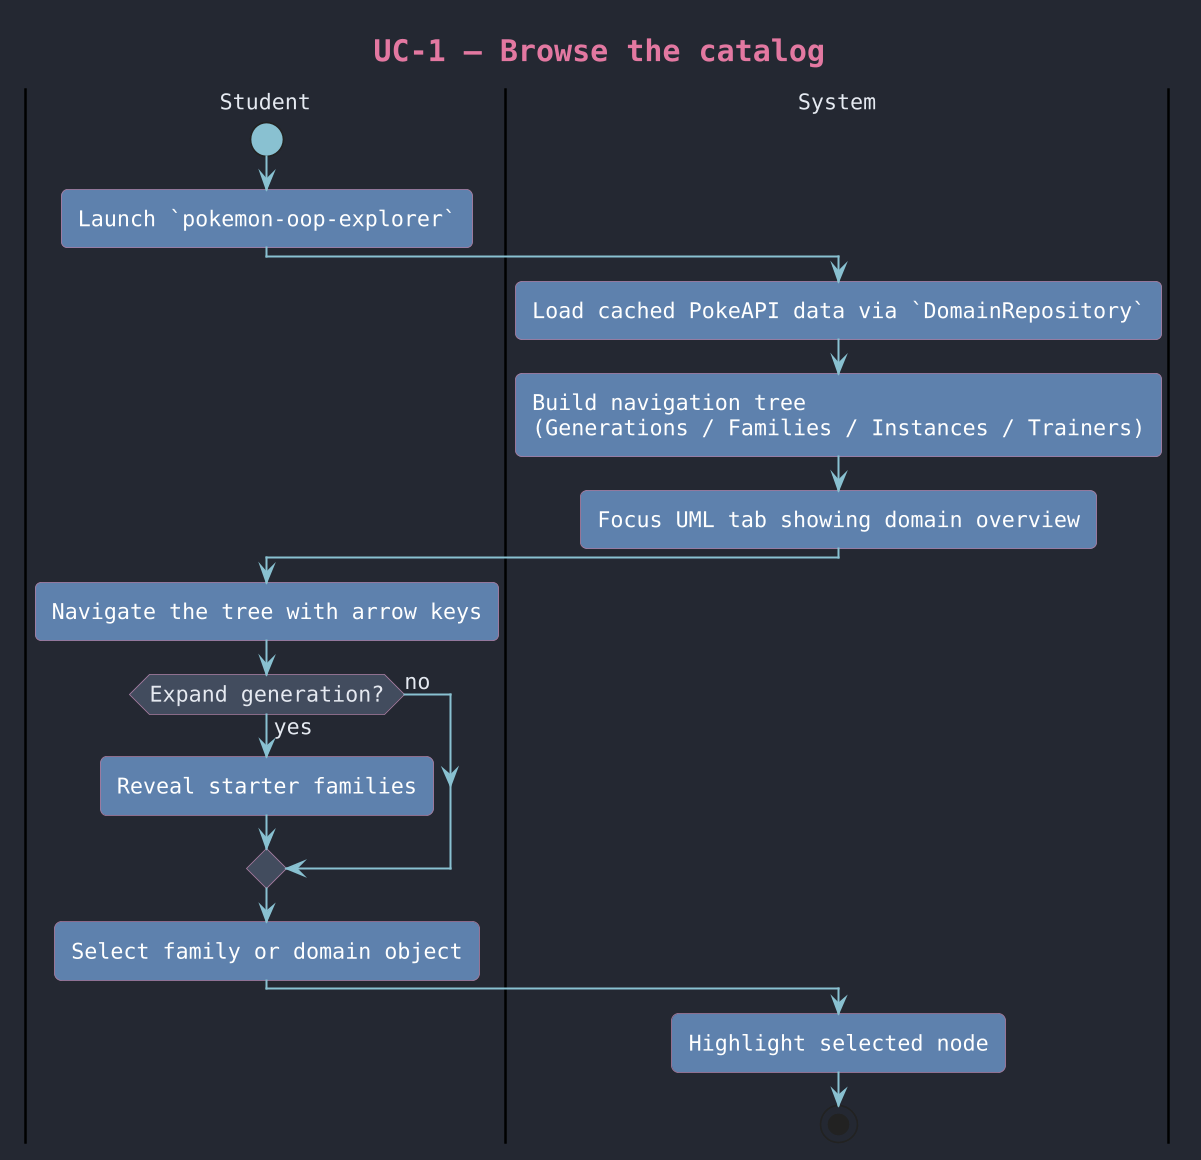
\includegraphics[width=\textwidth,keepaspectratio]{../docs/uml/use_cases/images/uc-1_browse_catalog.png}
\end{center}
\textit{UC-1 Browse catalog (zoom recommended).}

\begin{center}
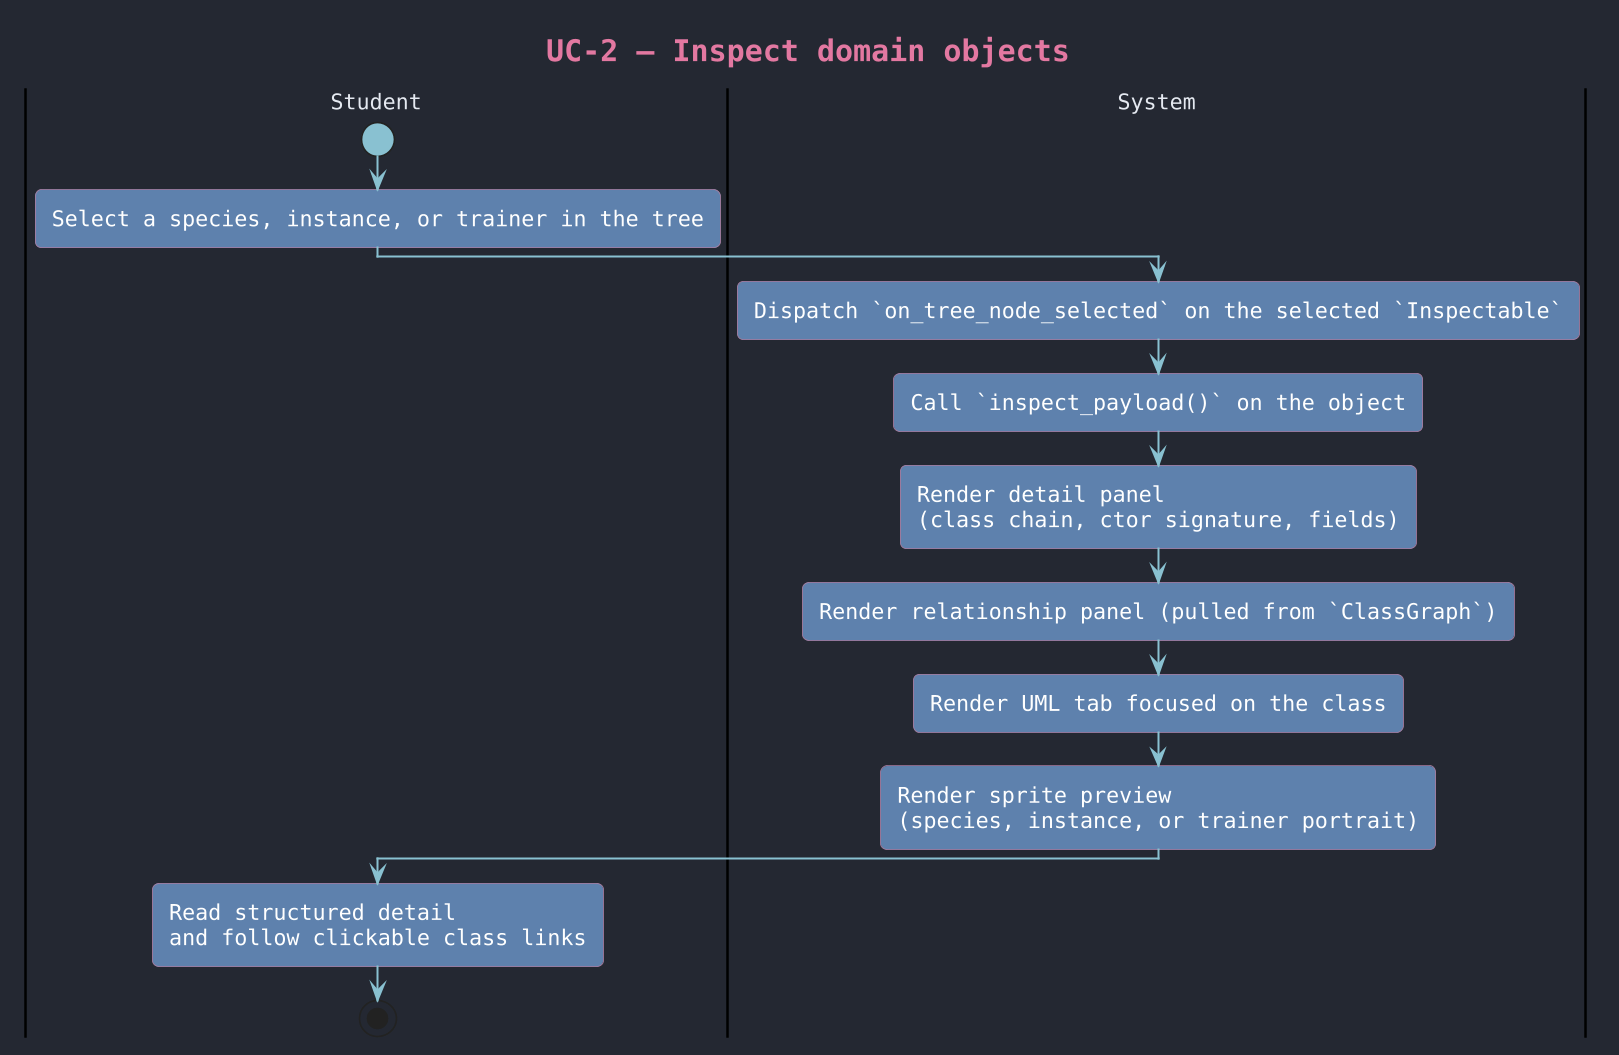
\includegraphics[width=\textwidth,keepaspectratio]{../docs/uml/use_cases/images/uc-2_inspect_domain.png}
\end{center}
\textit{UC-2 Inspect domain objects (zoom recommended).}

\begin{center}
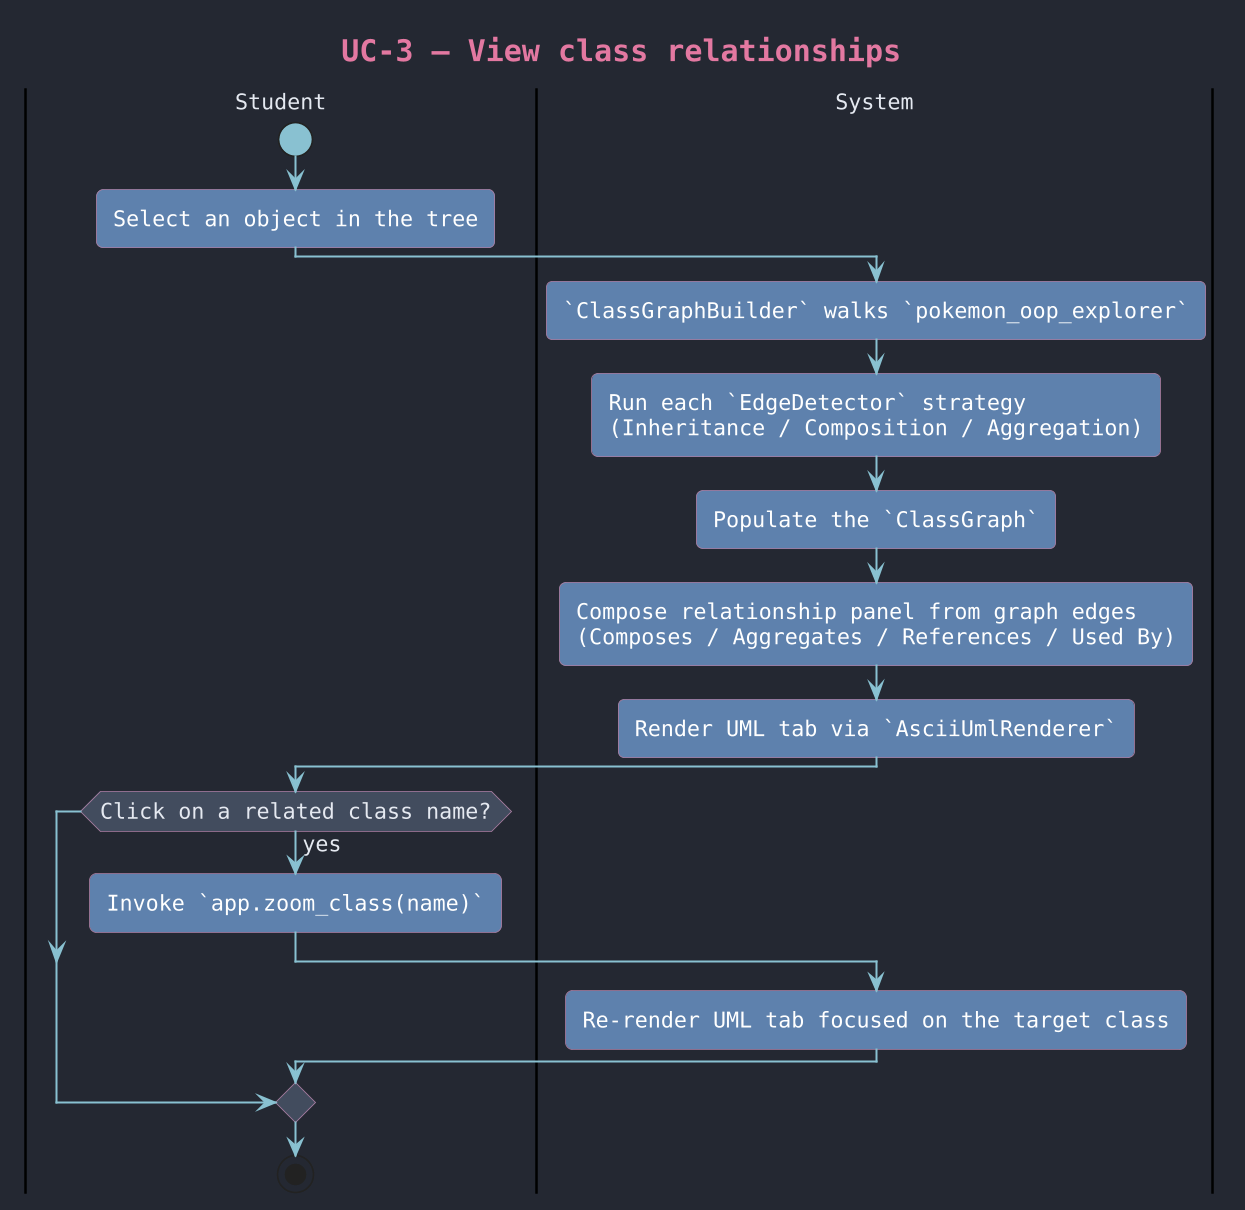
\includegraphics[width=\textwidth,keepaspectratio]{../docs/uml/use_cases/images/uc-3_class_relationships.png}
\end{center}
\textit{UC-3 View class relationships (zoom recommended).}

\begin{center}
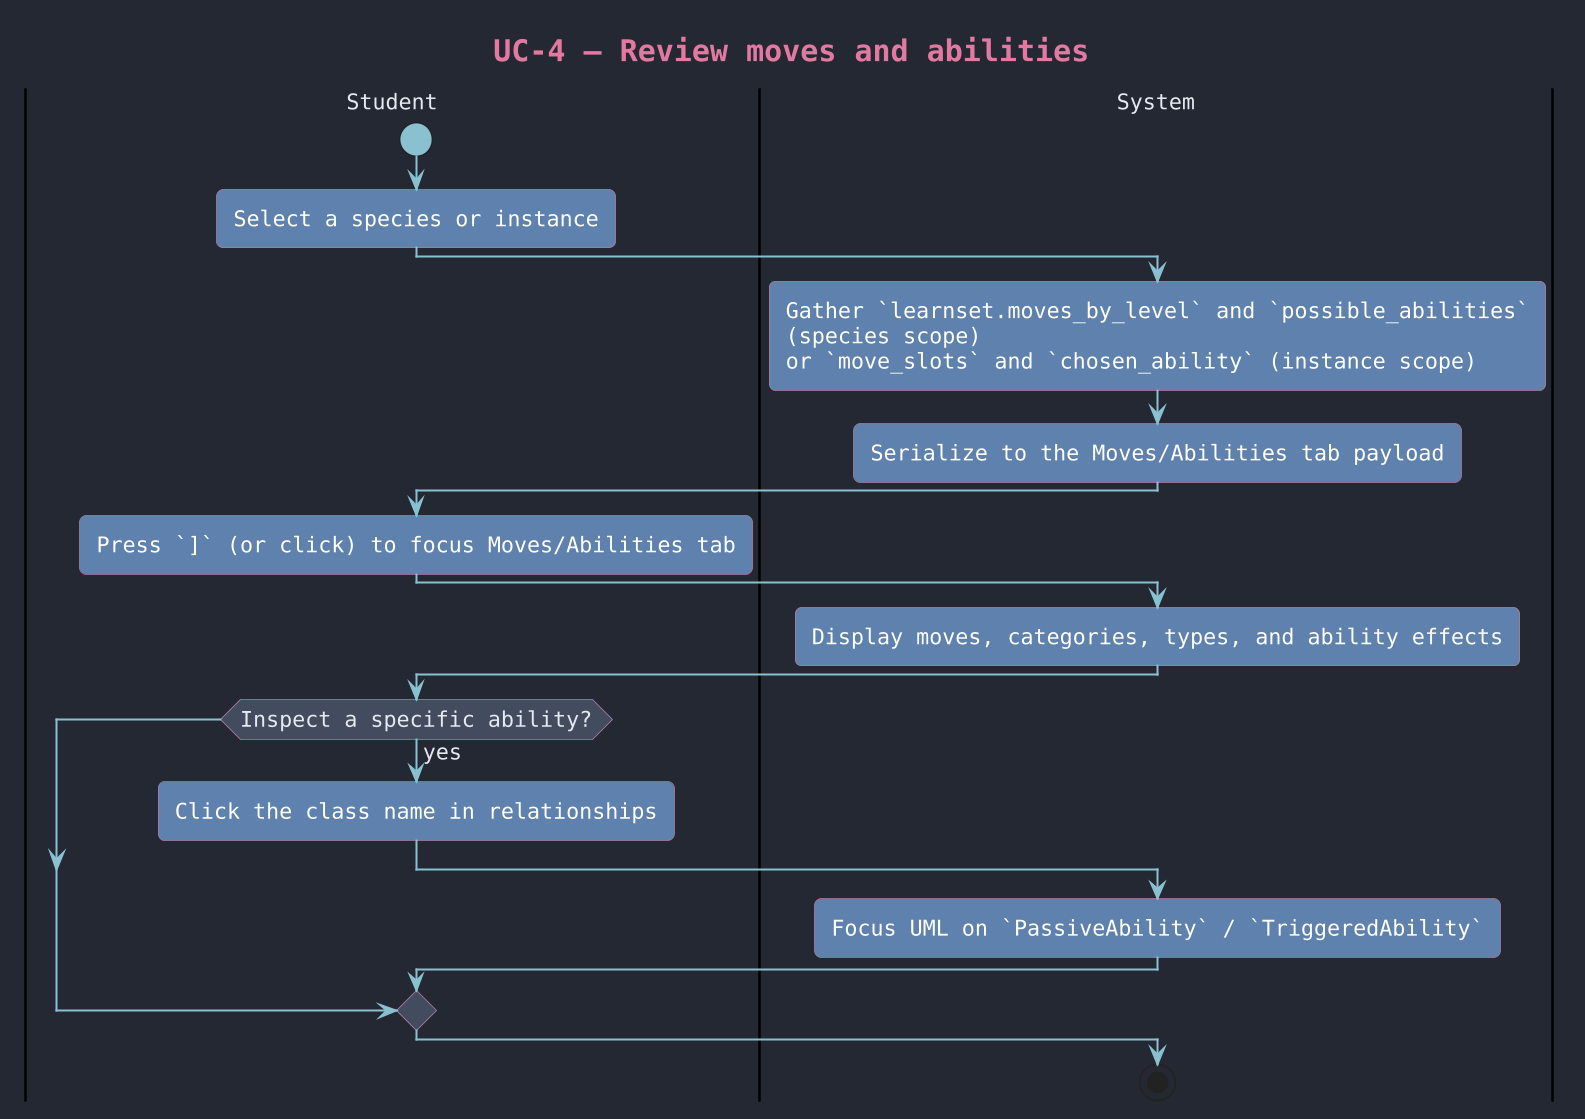
\includegraphics[width=\textwidth,keepaspectratio]{../docs/uml/use_cases/images/uc-4_moves_abilities.png}
\end{center}
\textit{UC-4 Review moves and abilities (zoom recommended).}

\begin{center}
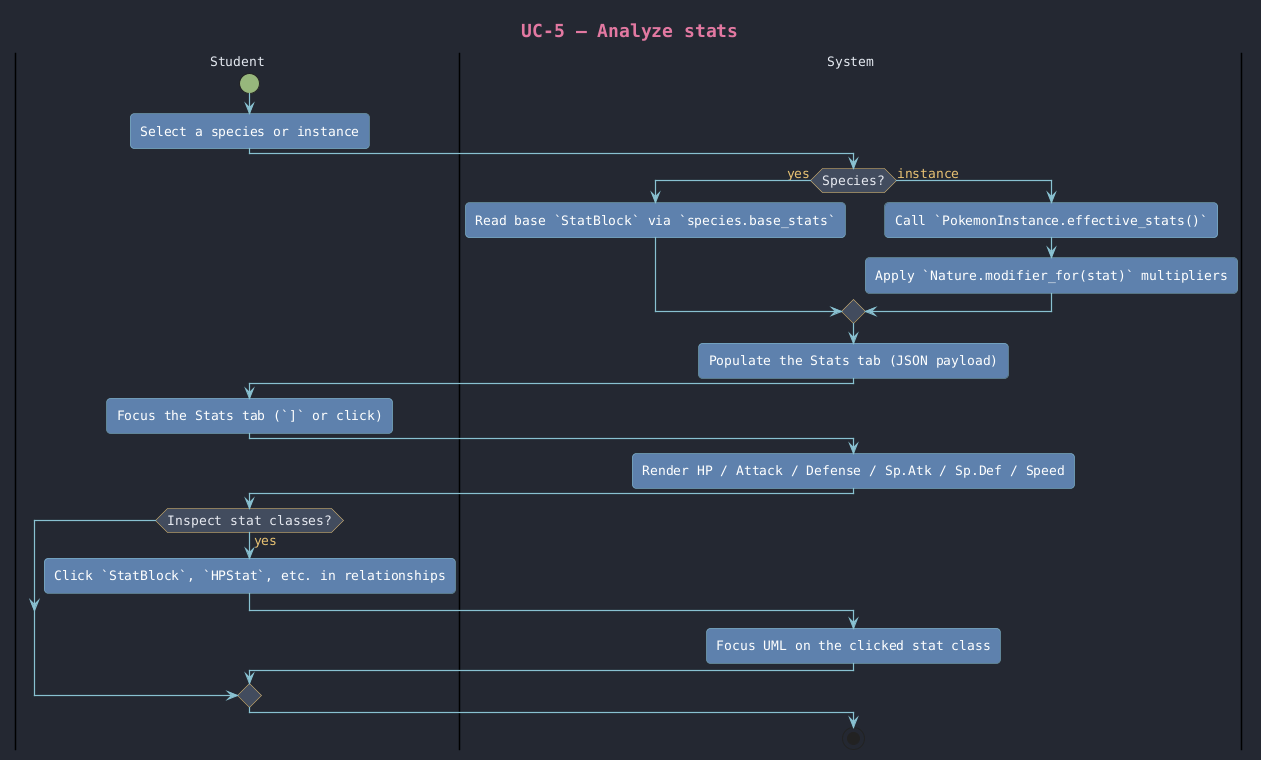
\includegraphics[width=\textwidth,keepaspectratio]{../docs/uml/use_cases/images/uc-5_analyze_stats.png}
\end{center}
\textit{UC-5 Analyze stats (zoom recommended).}

\begin{center}
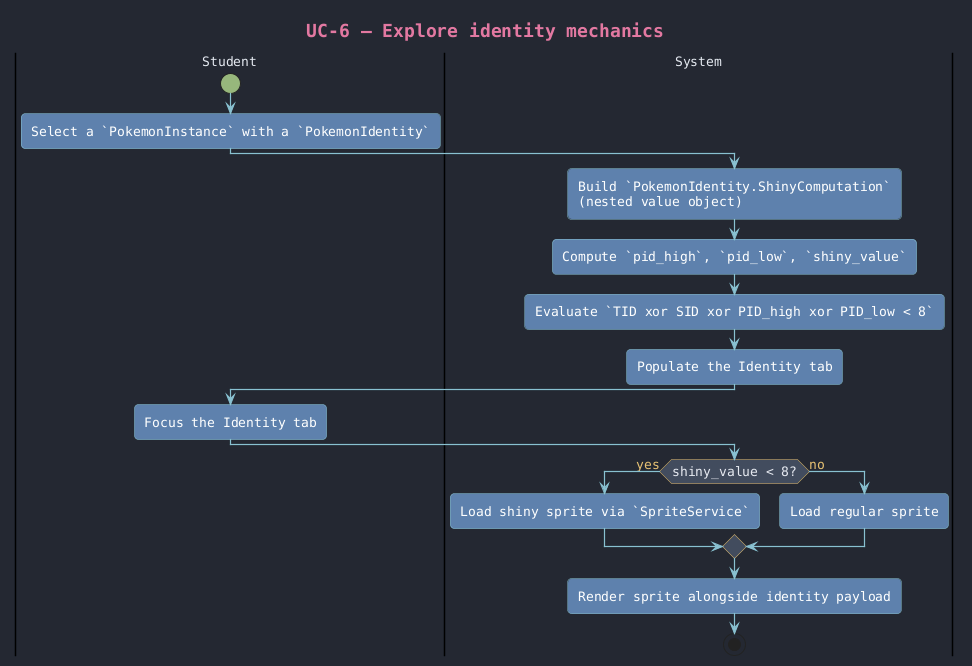
\includegraphics[width=\textwidth,keepaspectratio]{../docs/uml/use_cases/images/uc-6_identity_mechanics.png}
\end{center}
\textit{UC-6 Identity mechanics (zoom recommended).}

\begin{center}
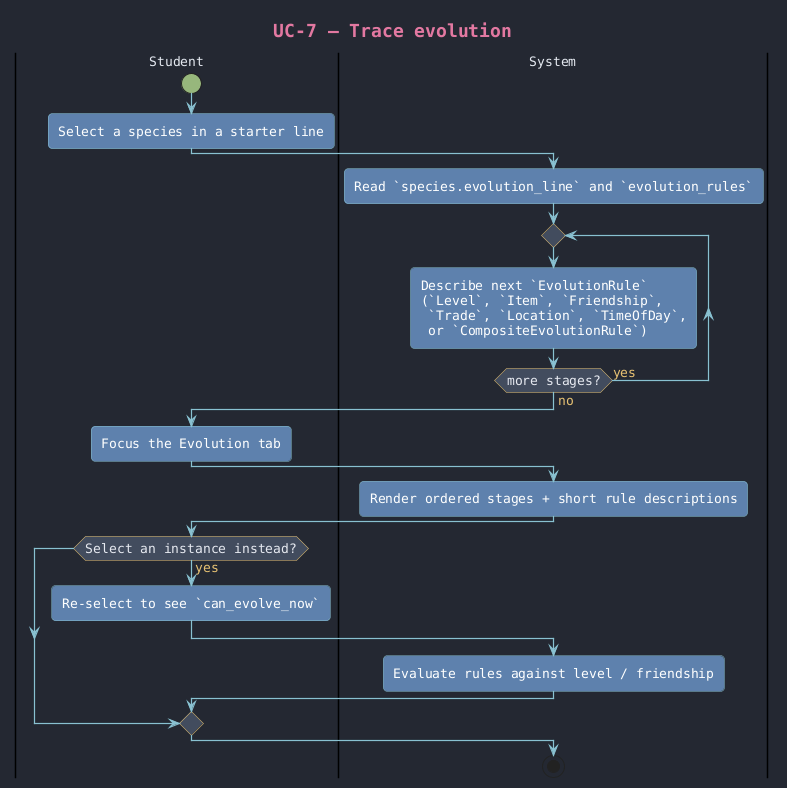
\includegraphics[width=\textwidth,keepaspectratio]{../docs/uml/use_cases/images/uc-7_trace_evolution.png}
\end{center}
\textit{UC-7 Trace evolution (zoom recommended).}

\begin{center}
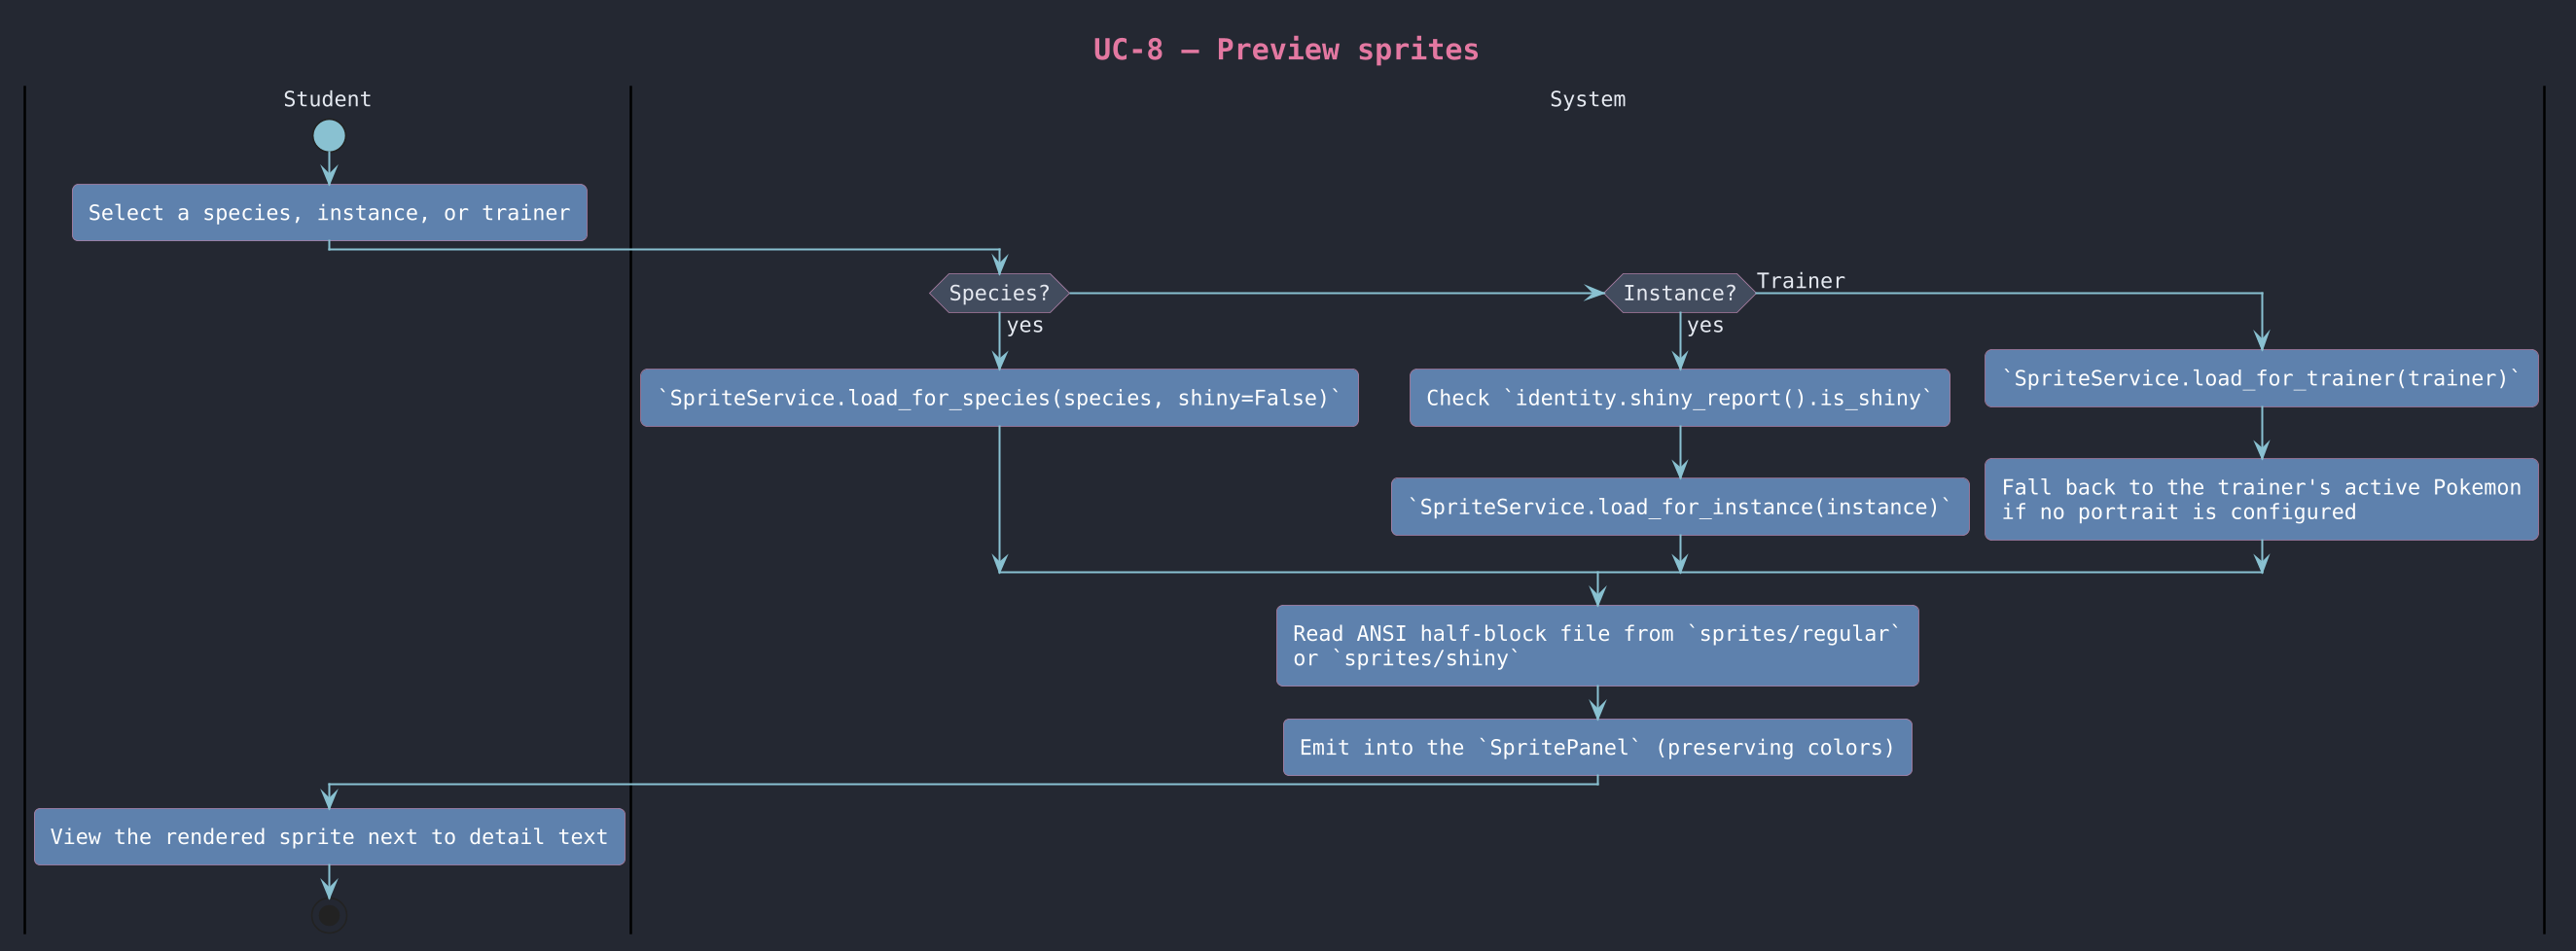
\includegraphics[width=\textwidth,keepaspectratio]{../docs/uml/use_cases/images/uc-8_preview_sprites.png}
\end{center}
\textit{UC-8 Preview sprites (zoom recommended).}

\newpage
\subsection*{Class Diagram}
\textit{Large detailed diagram; zoom strongly recommended. Source:
\texttt{docs/uml/class\_diagram/images/}.}

\begin{center}
\includegraphics[width=\textwidth,keepaspectratio]{../docs/uml/class_diagram/images/full_class_diagram.png}
\end{center}
\textit{Full class diagram (all discovered project classes with attributes and method signatures).}

\begin{center}
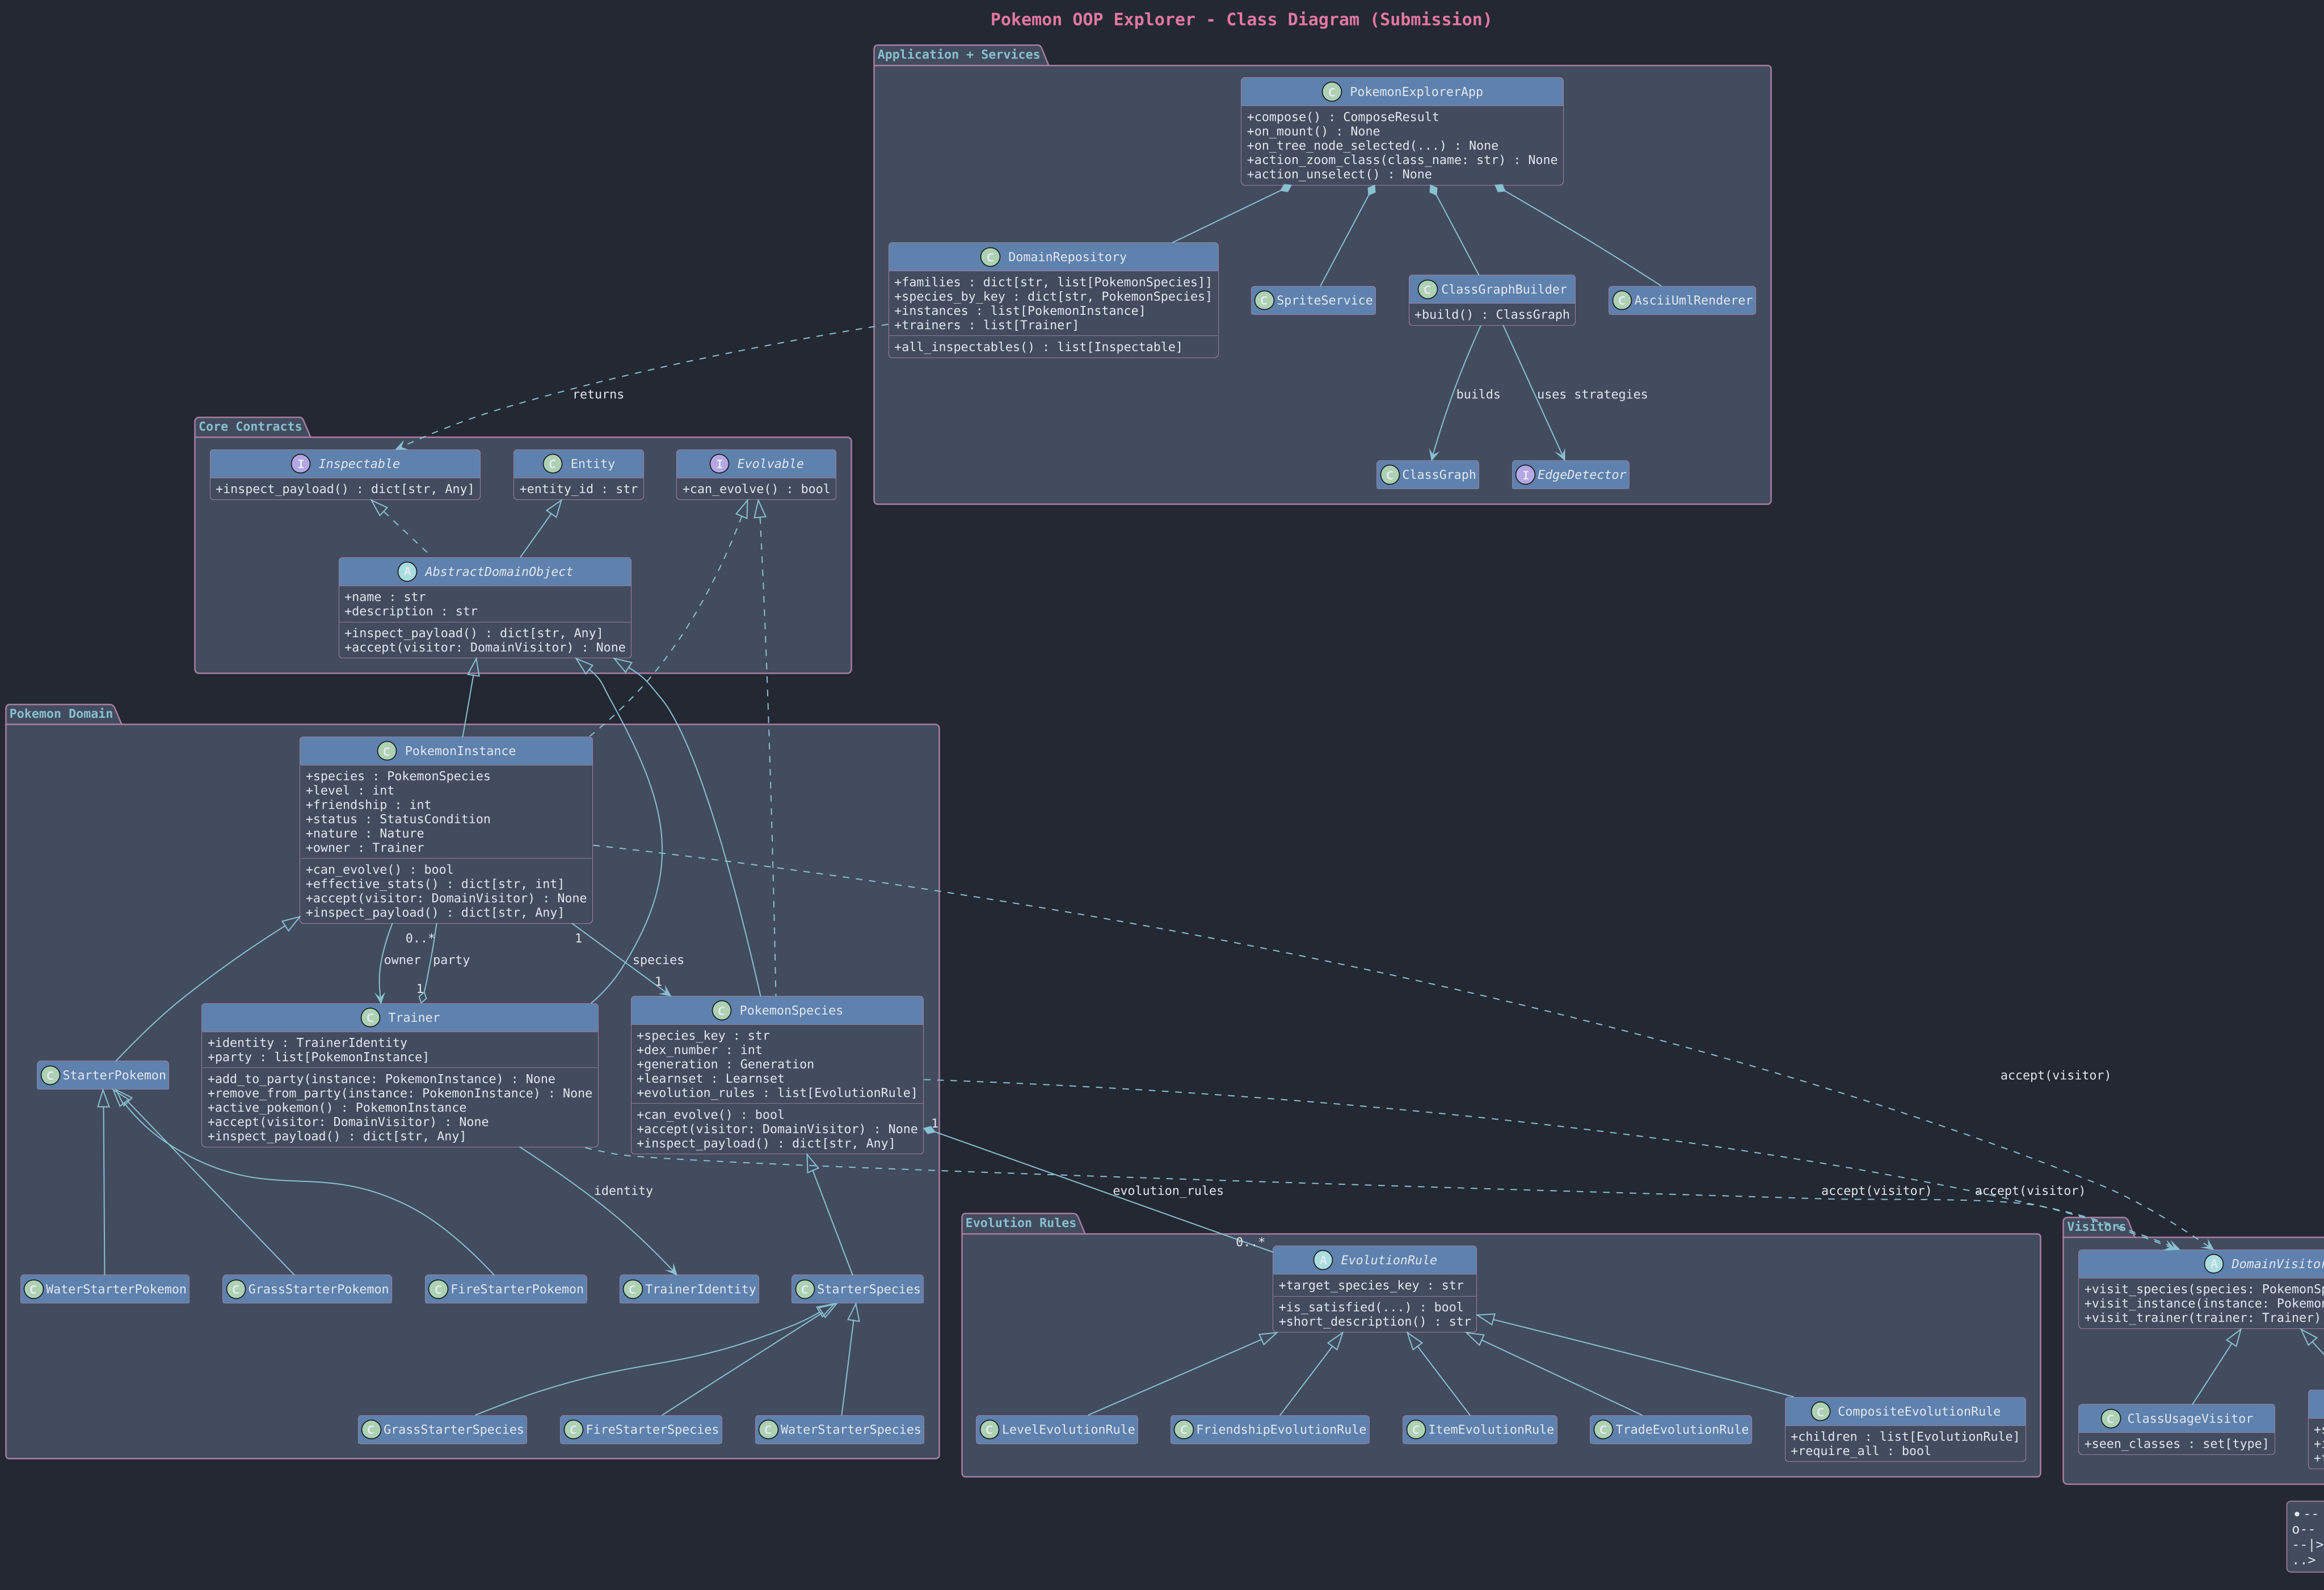
\includegraphics[width=\textwidth,keepaspectratio]{../docs/uml/class_diagram/images/domain_class_diagram.png}
\end{center}
\textit{Implementation-aligned class diagram.}

\newpage
\subsection*{Sequence Diagrams}
\textit{Most sequence diagrams are dense; zoom in or open the originals in
\texttt{docs/uml/sequences/images/}.}

\begin{center}
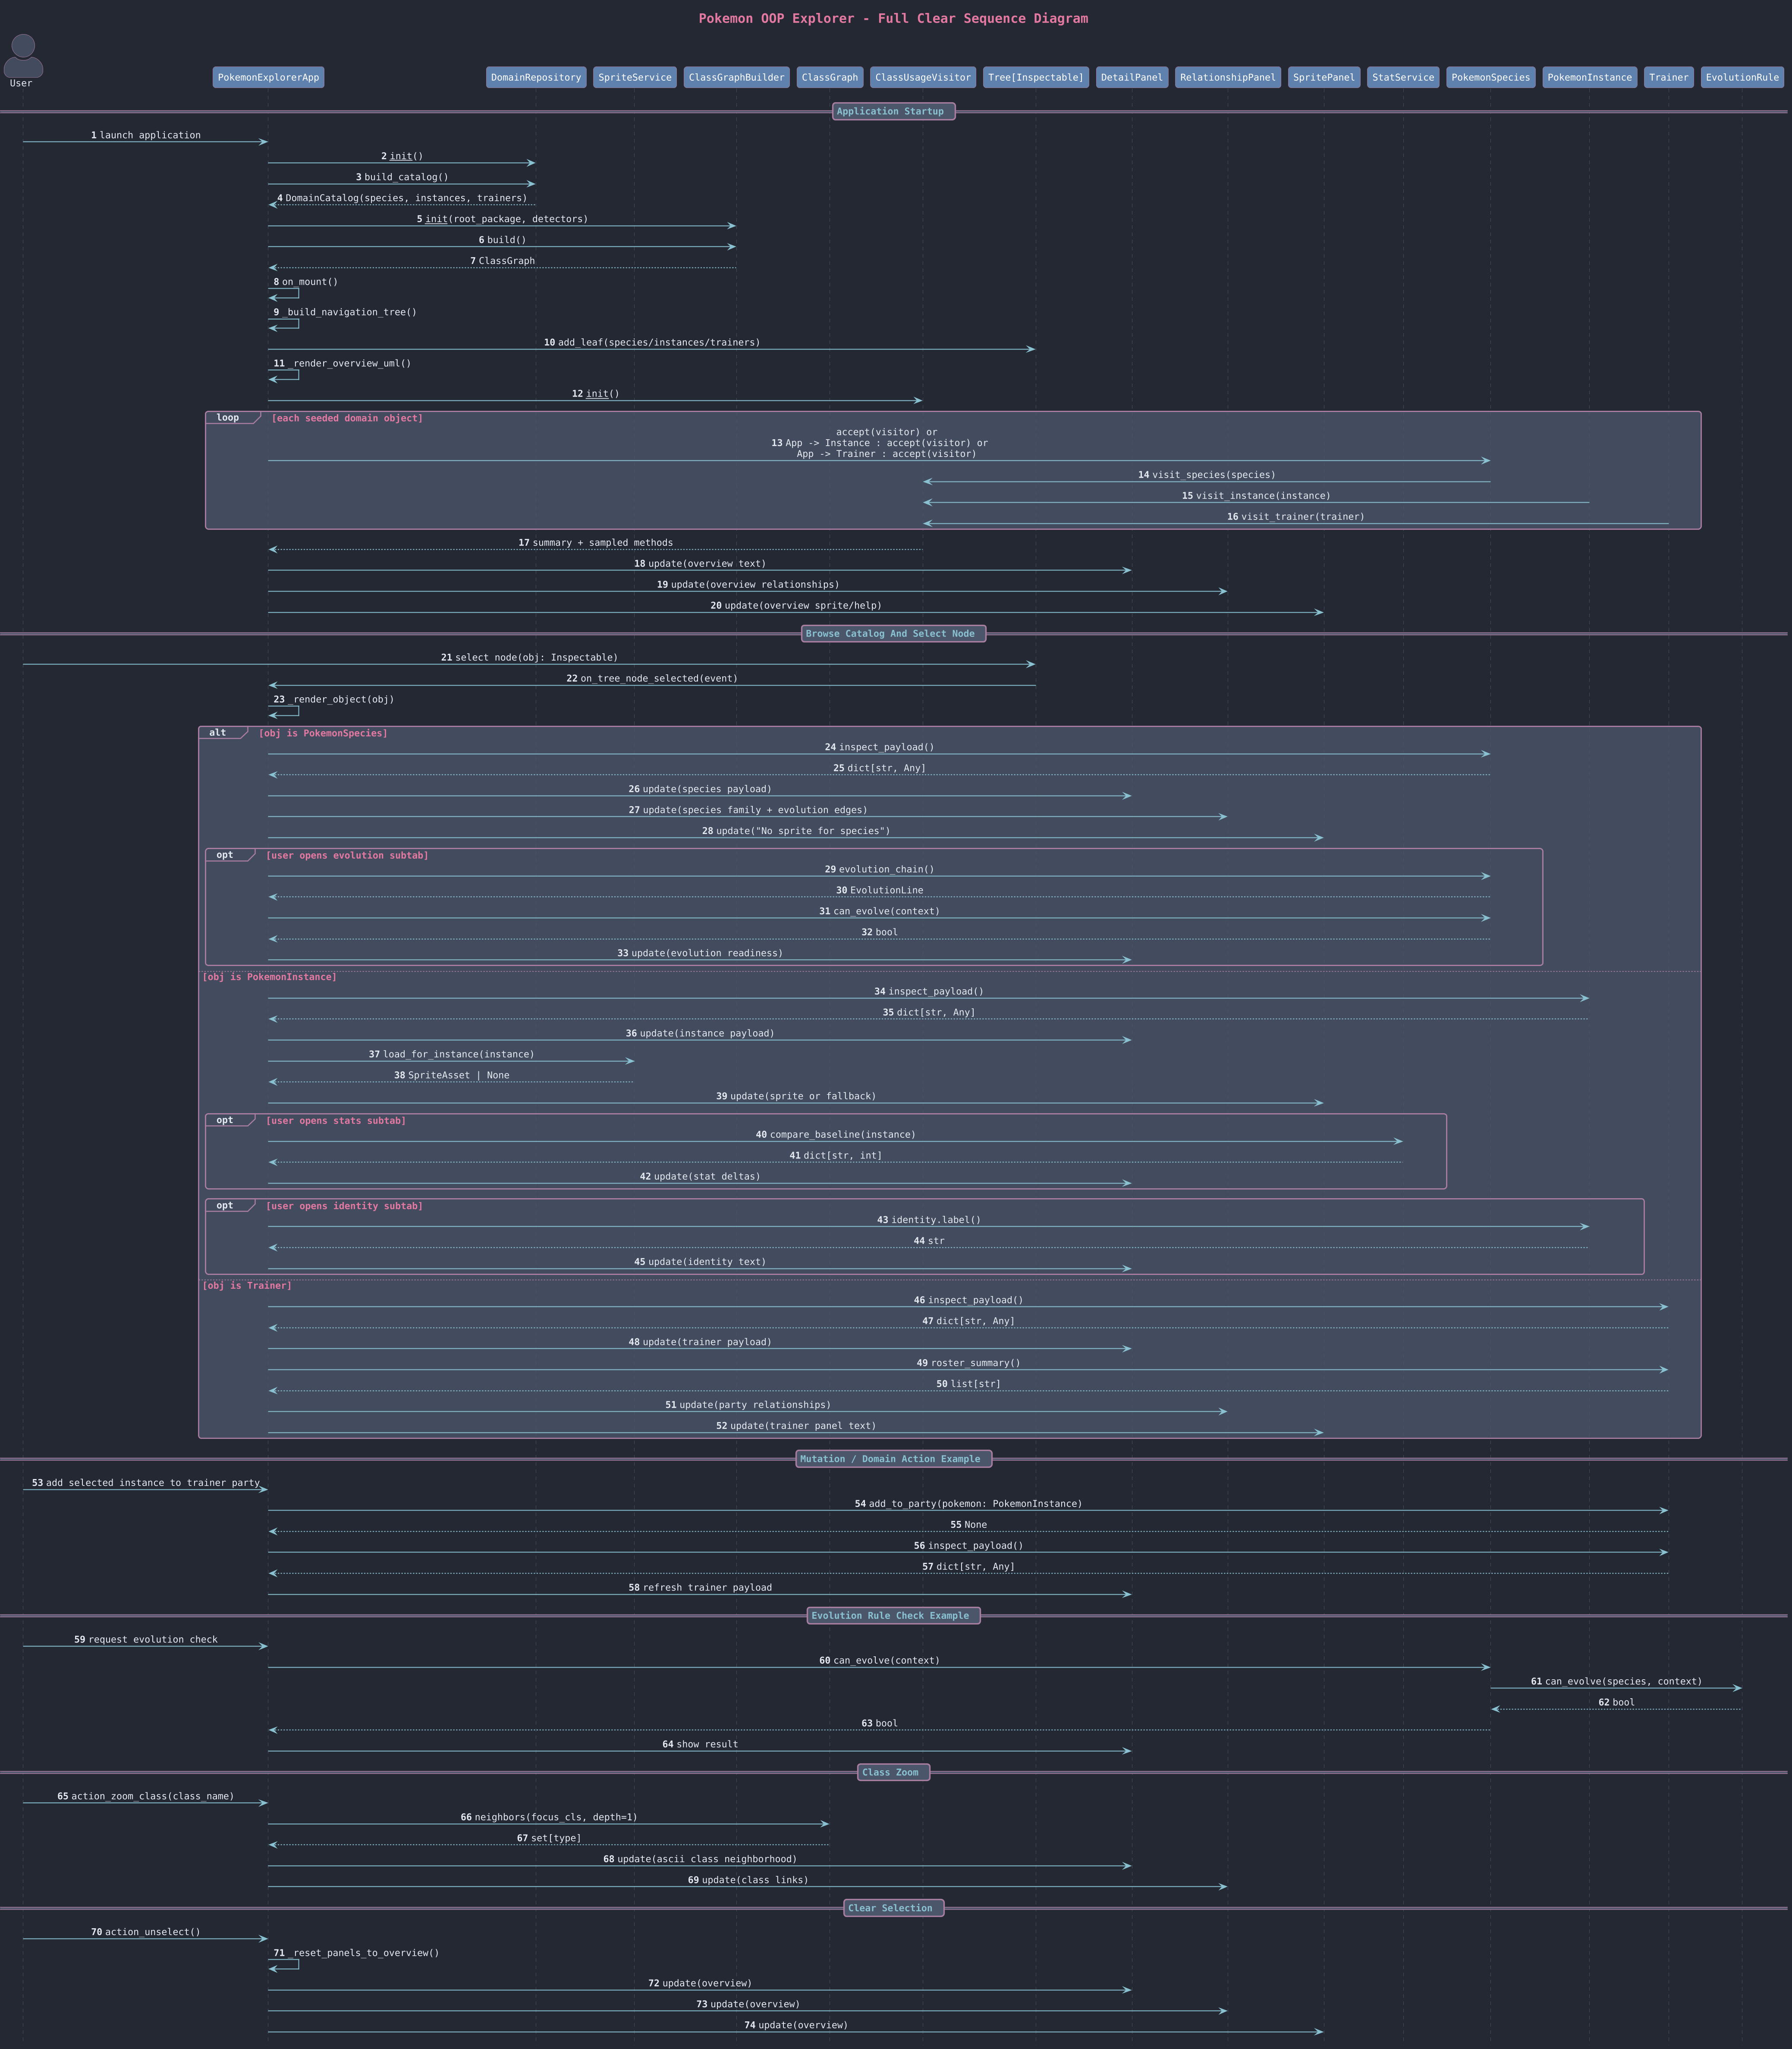
\includegraphics[width=\textwidth,keepaspectratio]{../docs/uml/sequences/images/full_sequence_diagram.png}
\end{center}
\textit{Full clear sequence diagram: startup, selection, rendering, domain action, and reset flow.}

\begin{center}
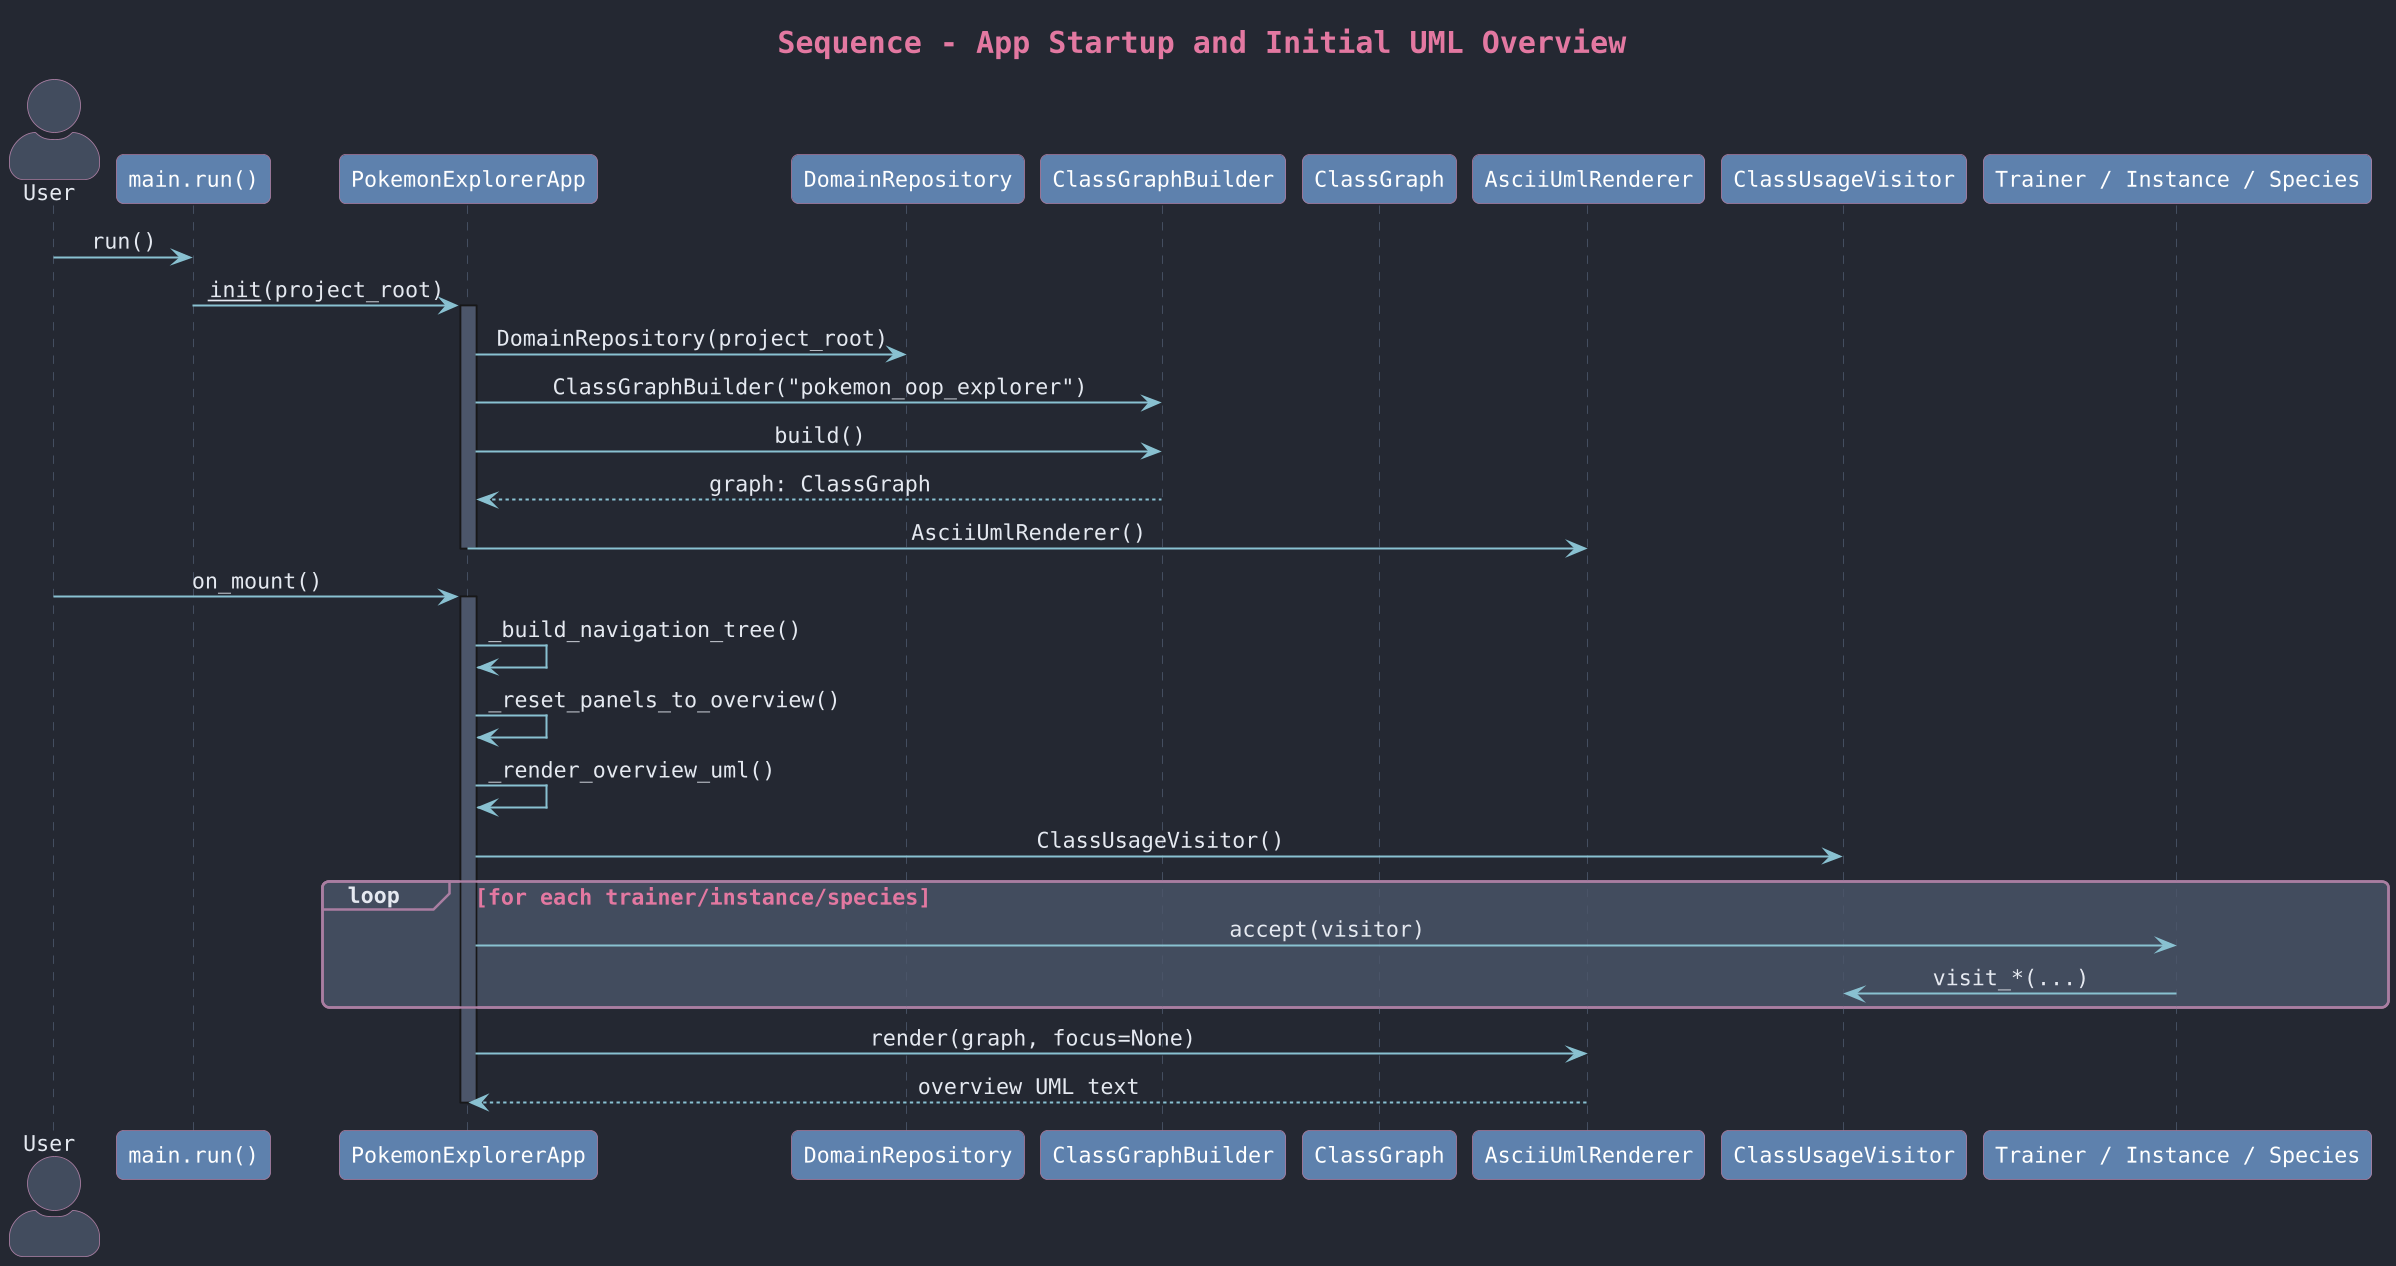
\includegraphics[width=\textwidth,keepaspectratio]{../docs/uml/sequences/images/seq_1_app_startup.png}
\end{center}
\textit{Sequence 1: app startup and initial UML overview (zoom recommended).}

\begin{center}
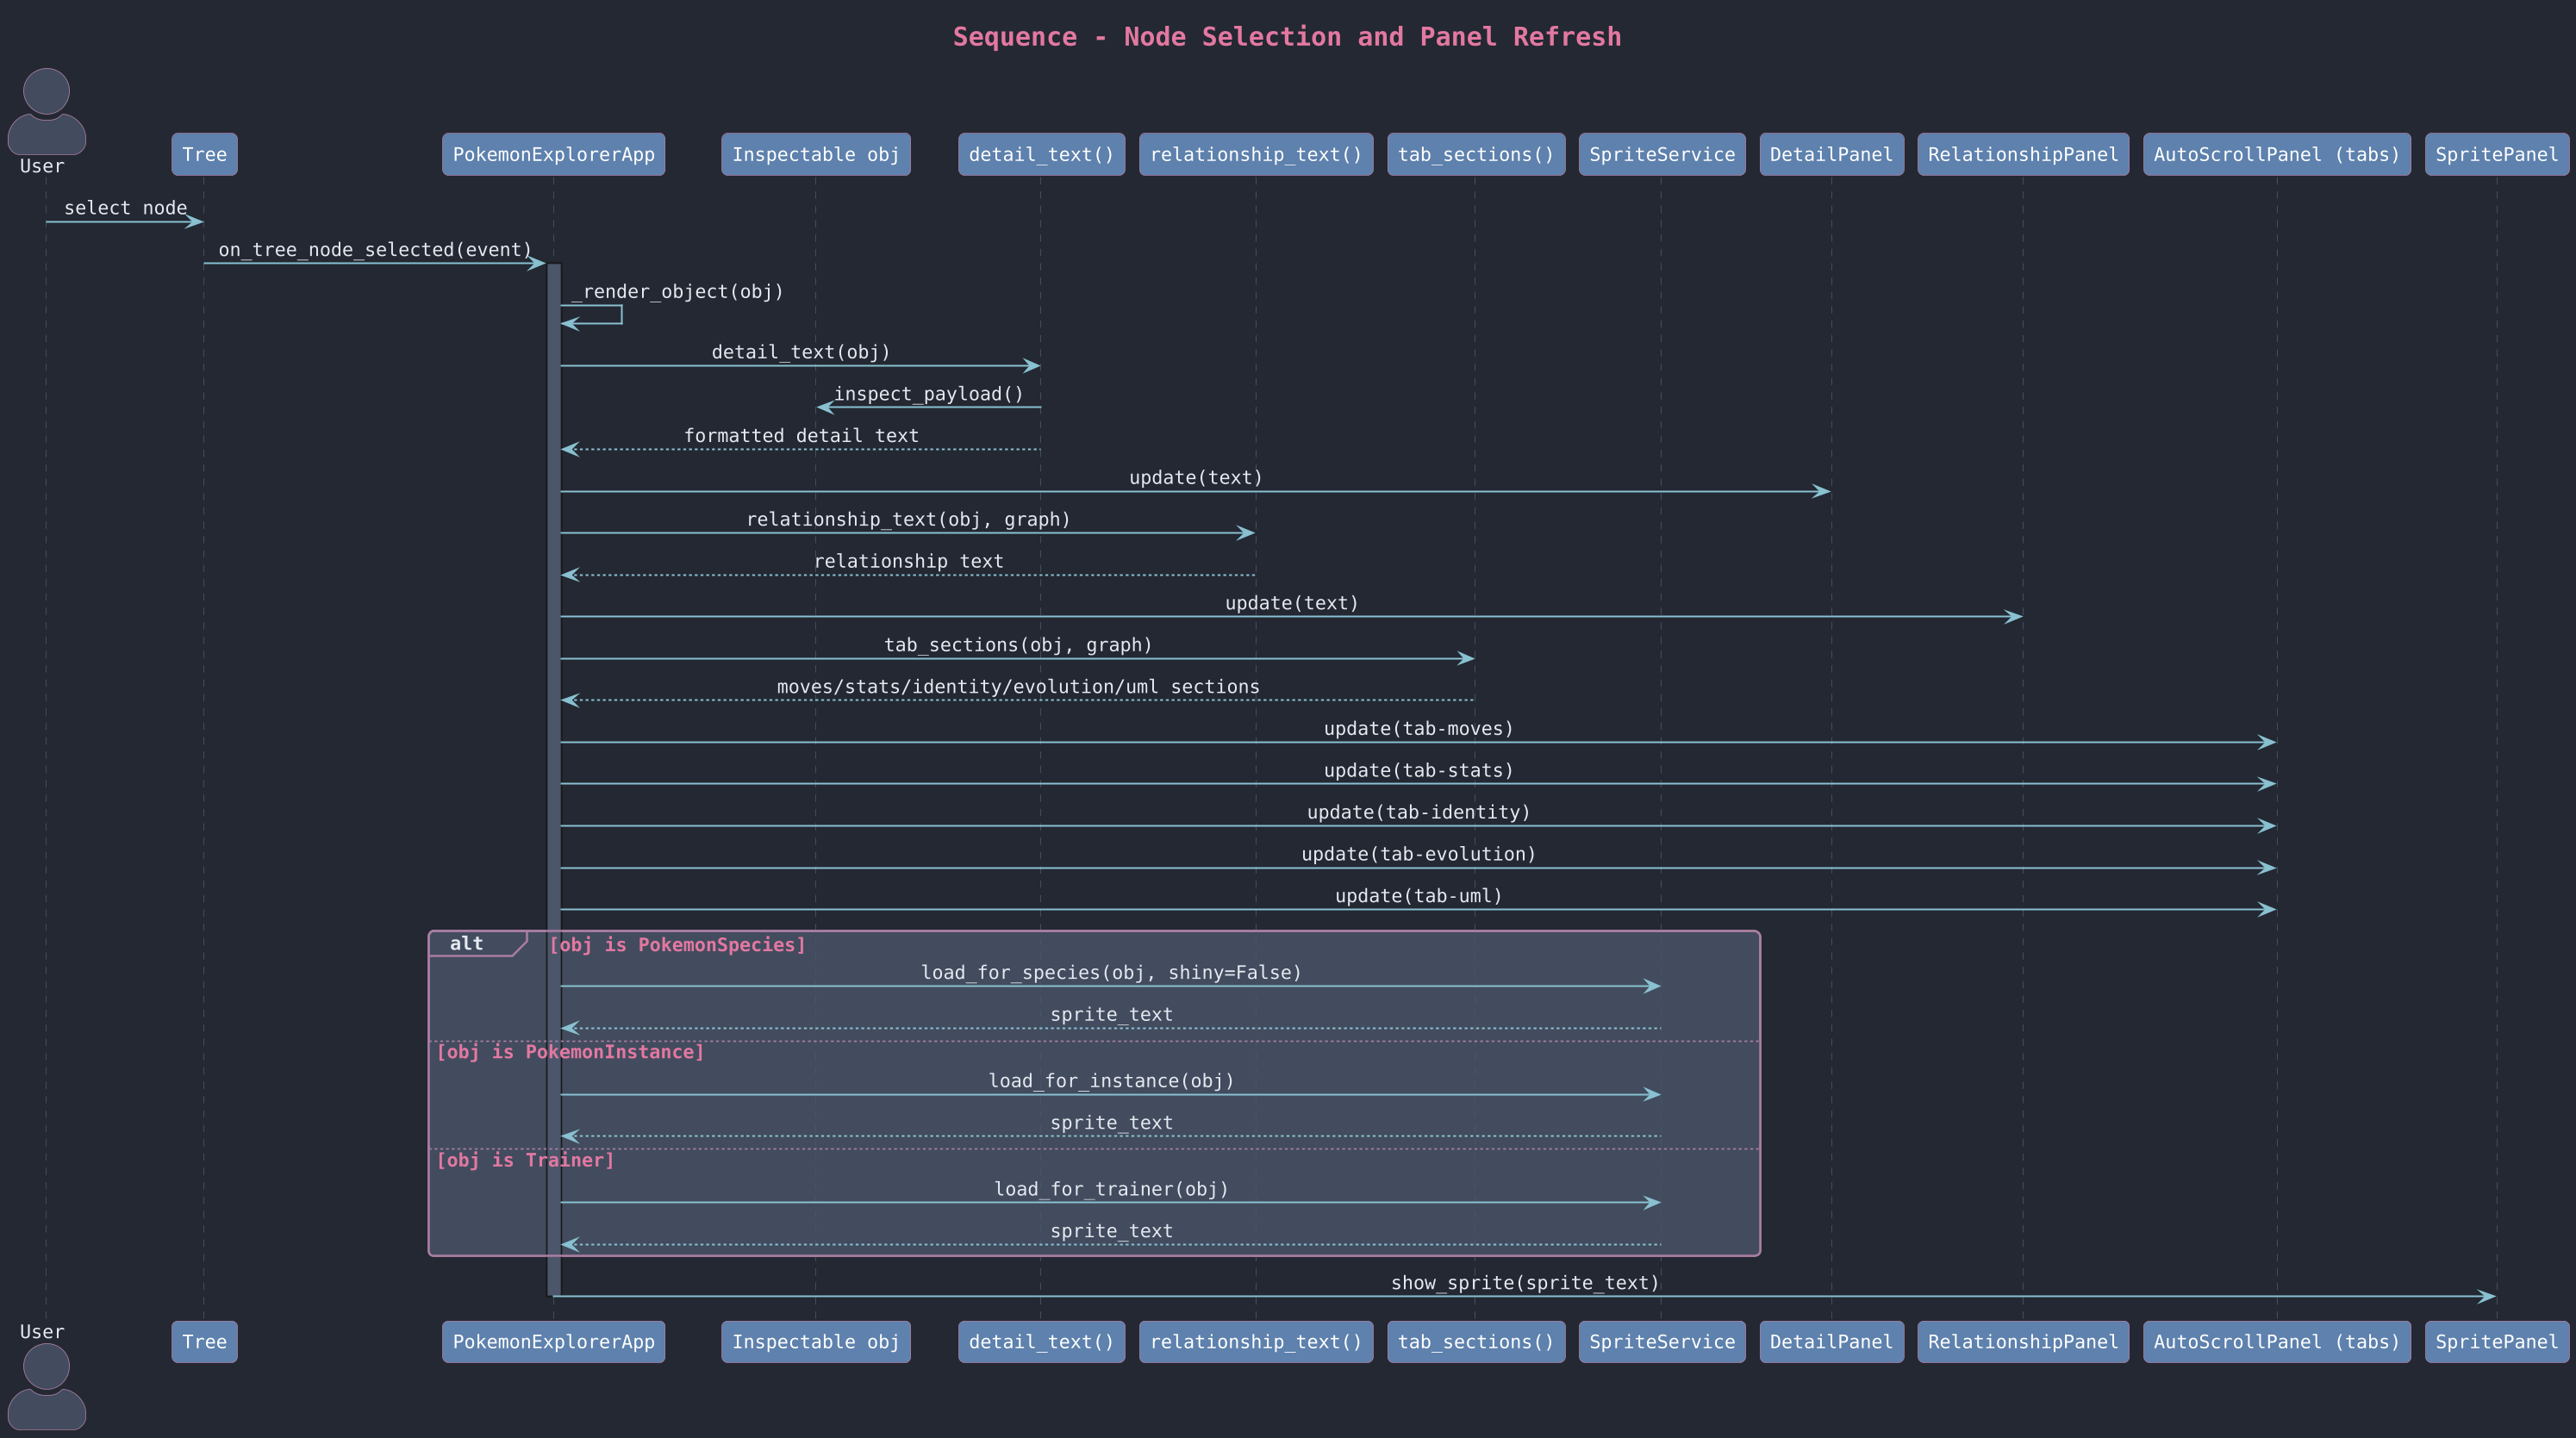
\includegraphics[width=\textwidth,keepaspectratio]{../docs/uml/sequences/images/seq_2_node_selection_refresh.png}
\end{center}
\textit{Sequence 2: node selection and panel refresh (zoom recommended).}

\begin{center}
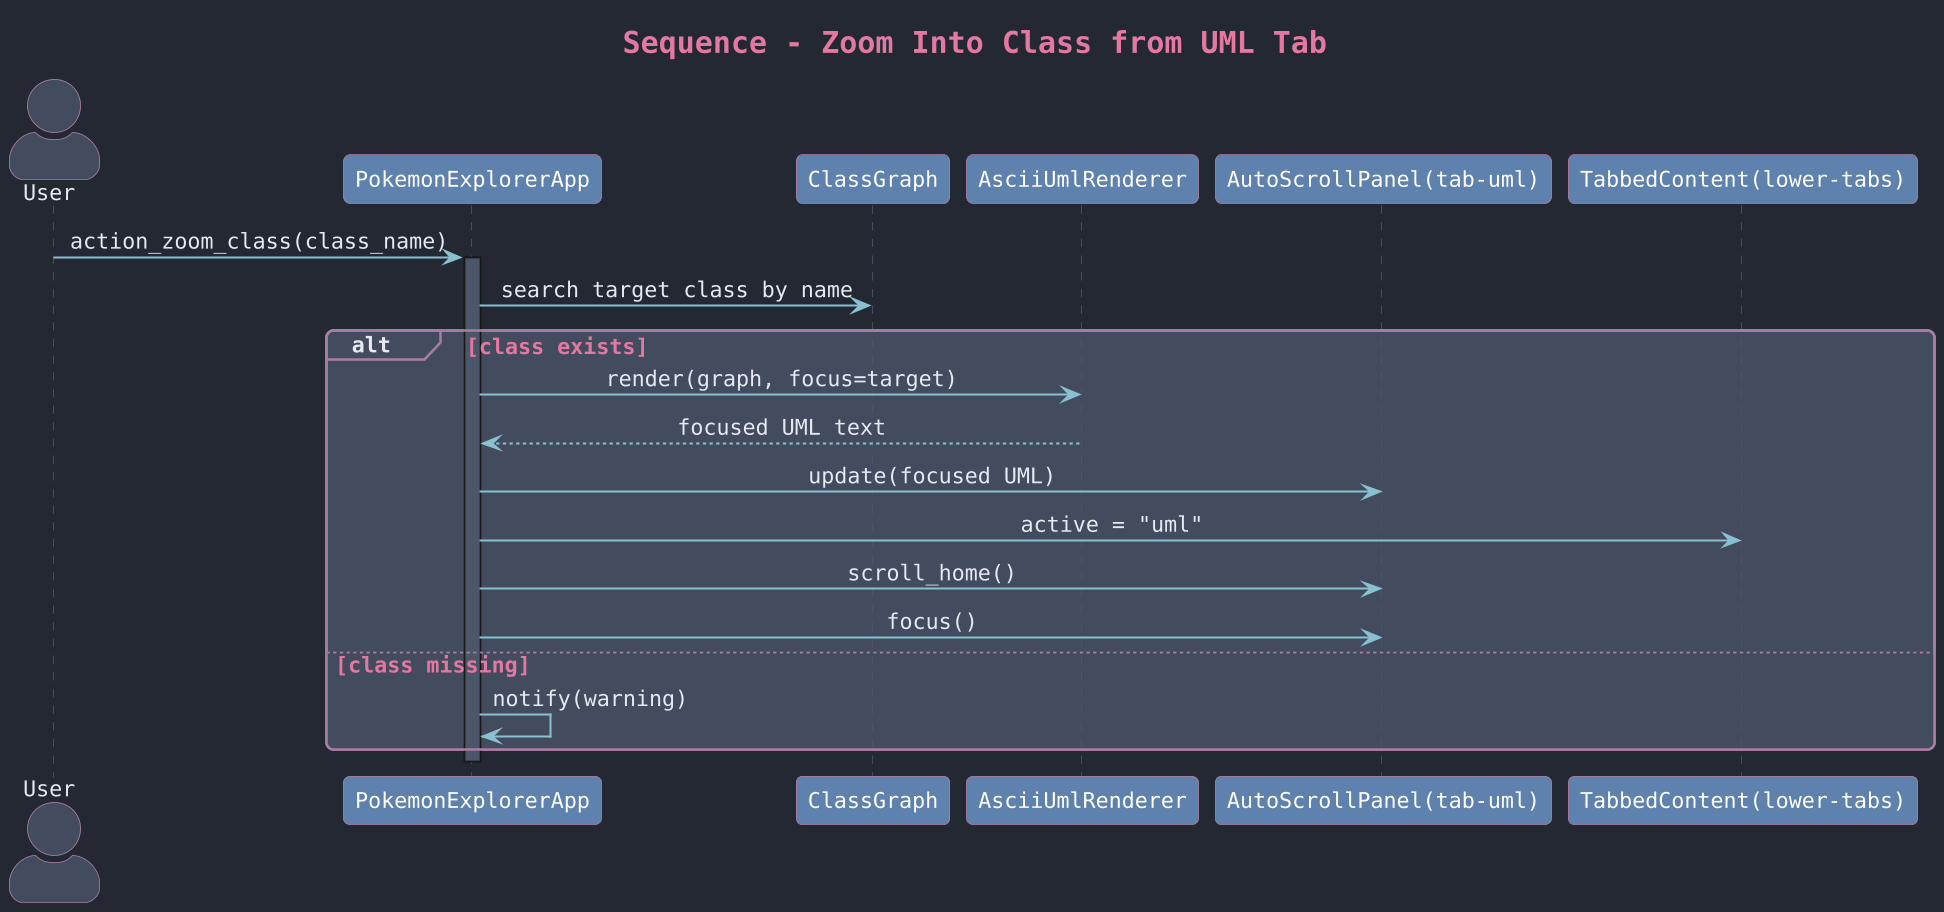
\includegraphics[width=\textwidth,keepaspectratio]{../docs/uml/sequences/images/seq_3_zoom_class.png}
\end{center}
\textit{Sequence 3: zoom class interaction.}

\begin{center}
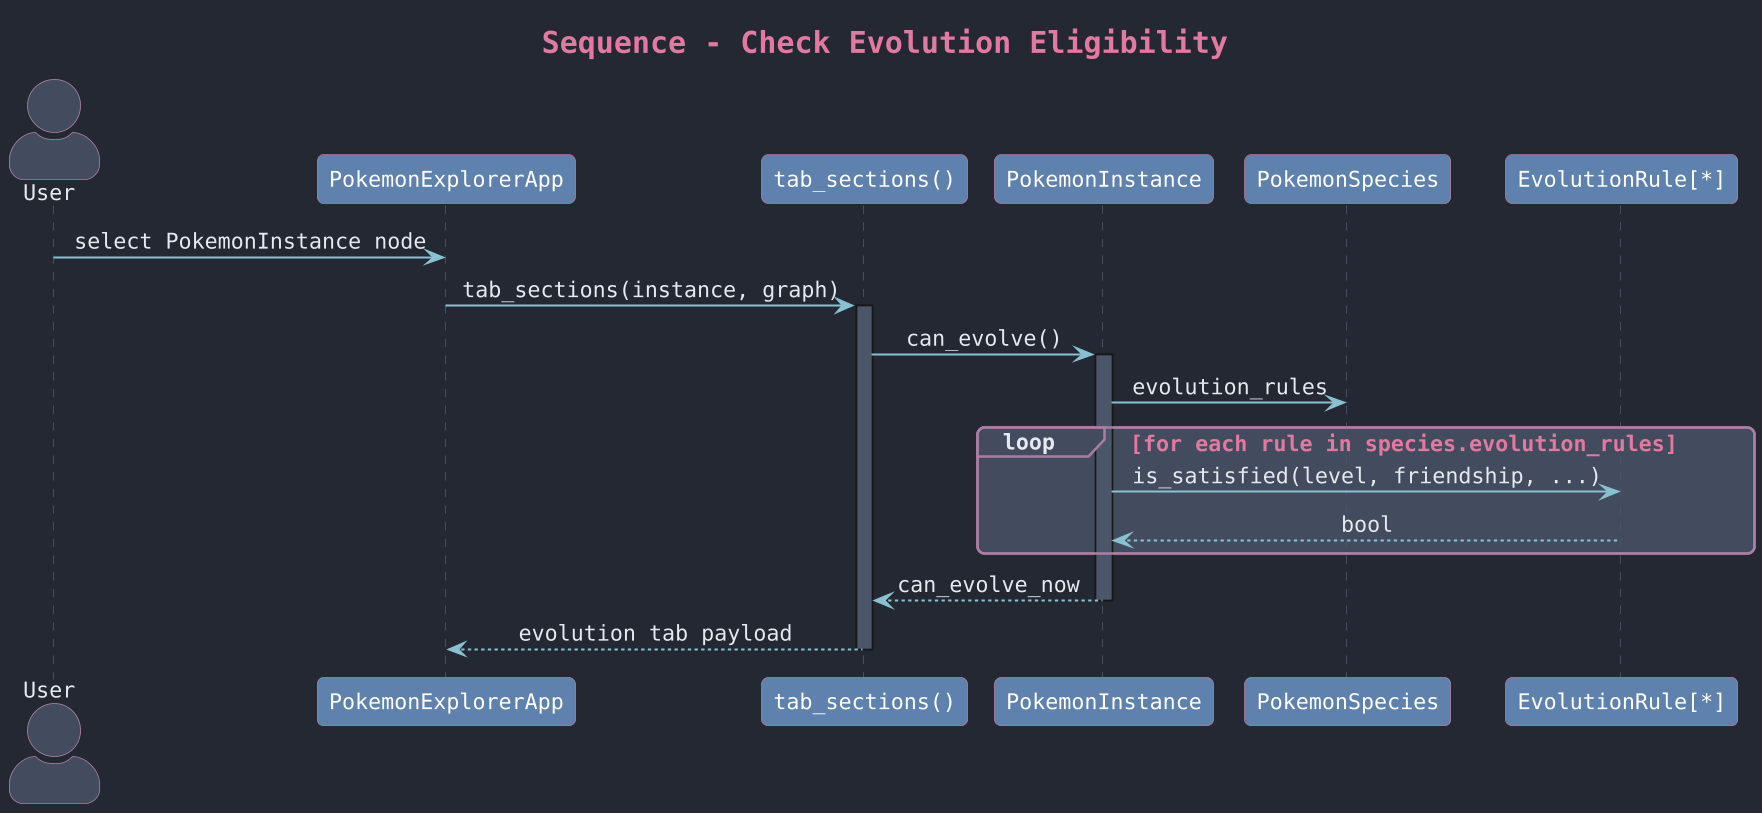
\includegraphics[width=\textwidth,keepaspectratio]{../docs/uml/sequences/images/seq_4_evolution_check.png}
\end{center}
\textit{Sequence 4: evolution eligibility check.}

\begin{center}
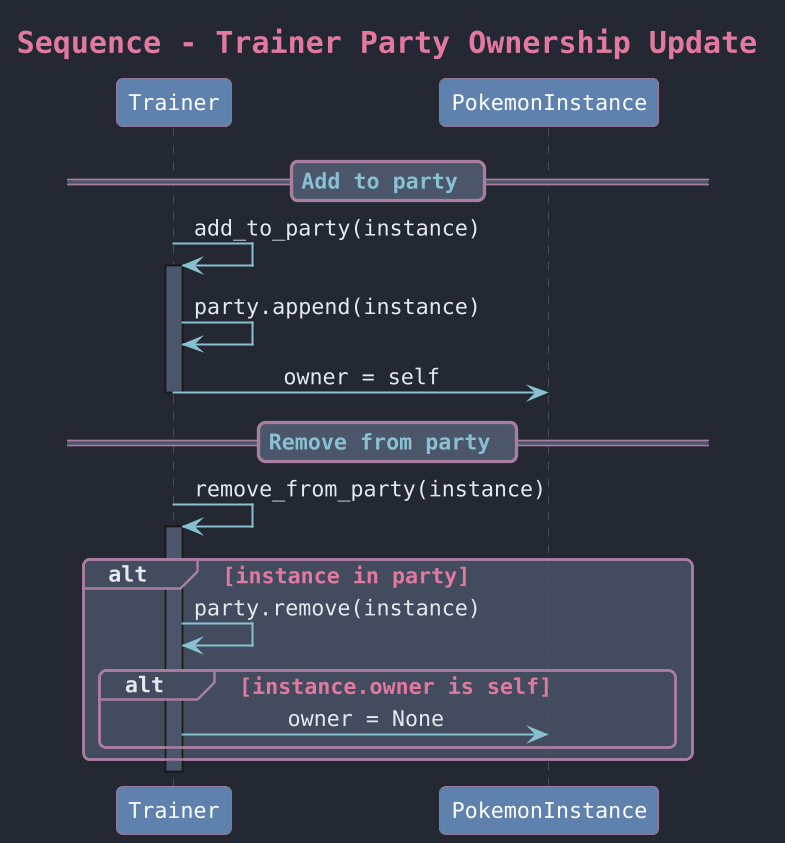
\includegraphics[width=\textwidth,keepaspectratio]{../docs/uml/sequences/images/seq_5_trainer_party_update.png}
\end{center}
\textit{Sequence 5: trainer party update (zoom recommended).}

\begin{center}
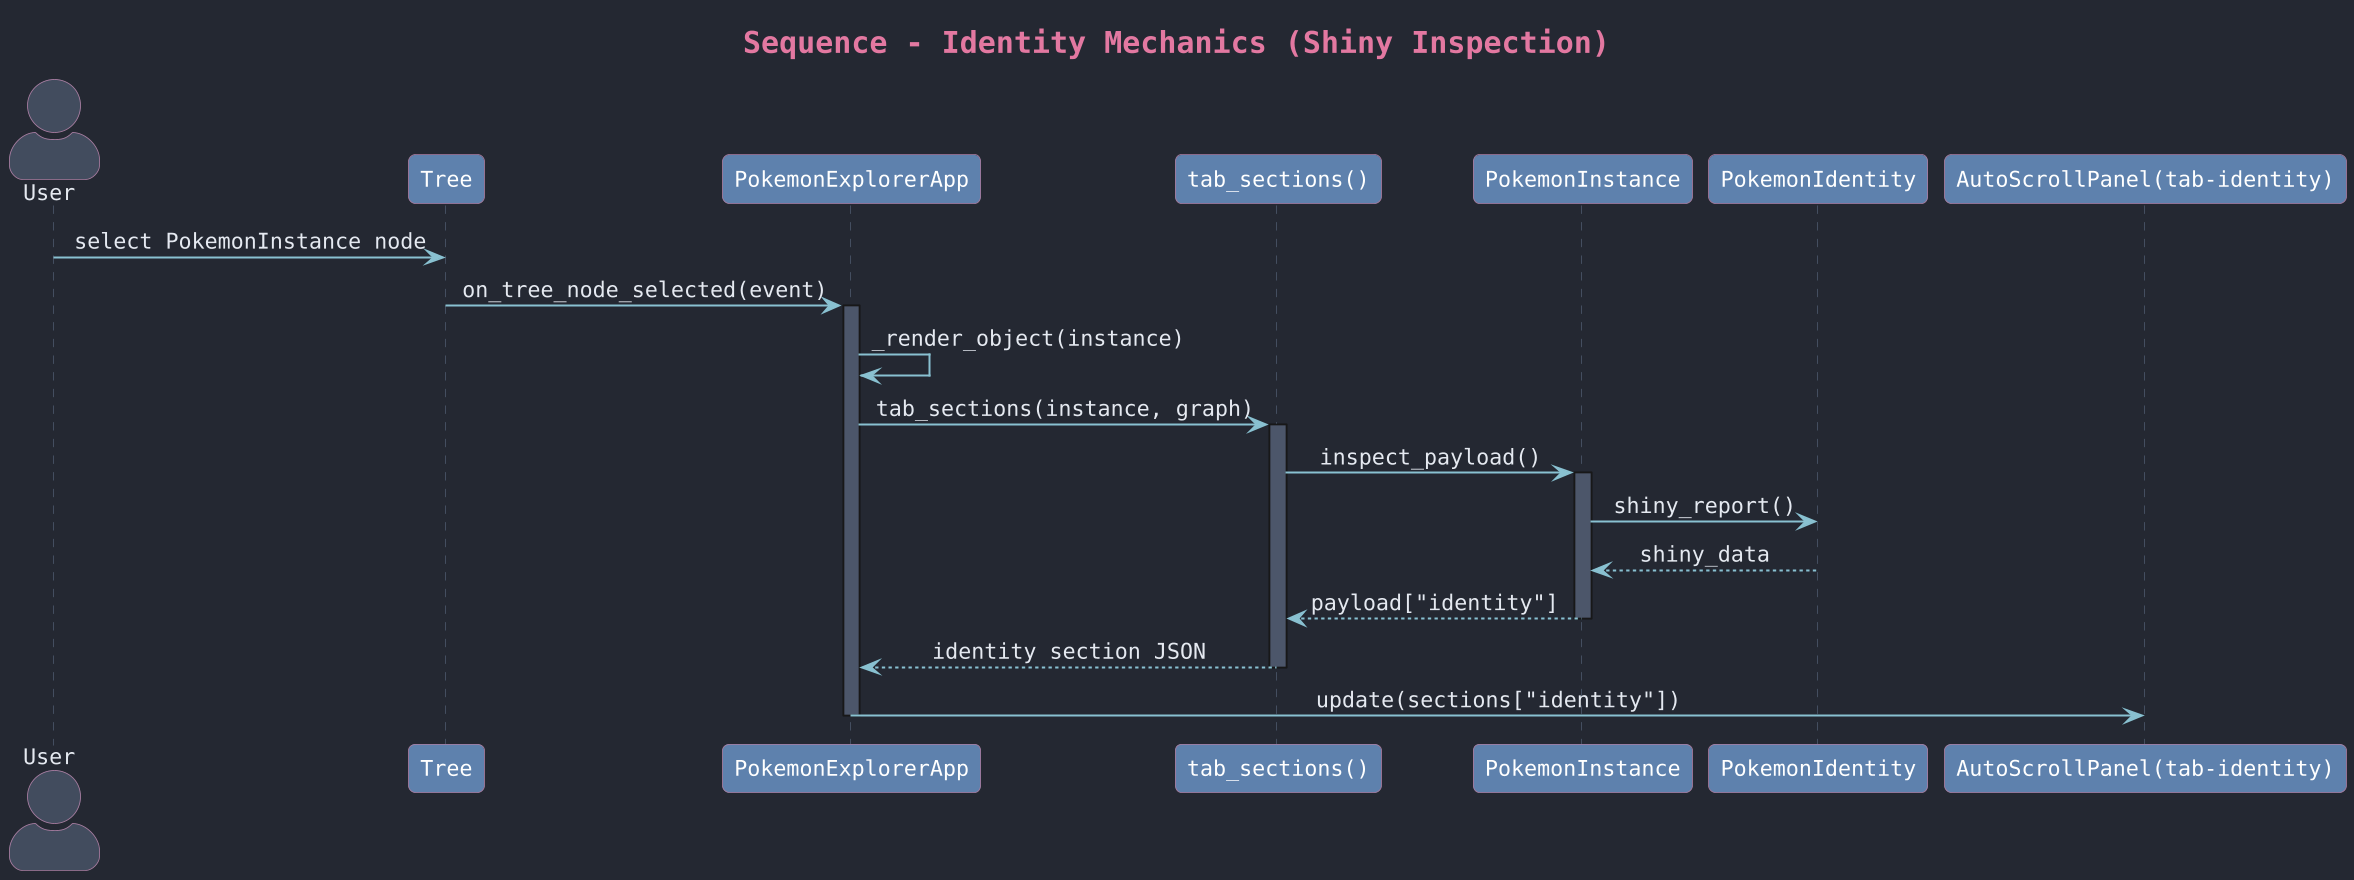
\includegraphics[width=\textwidth,keepaspectratio]{../docs/uml/sequences/images/seq_6_identity_mechanics.png}
\end{center}
\textit{Sequence 6: identity mechanics (zoom recommended).}

\begin{center}
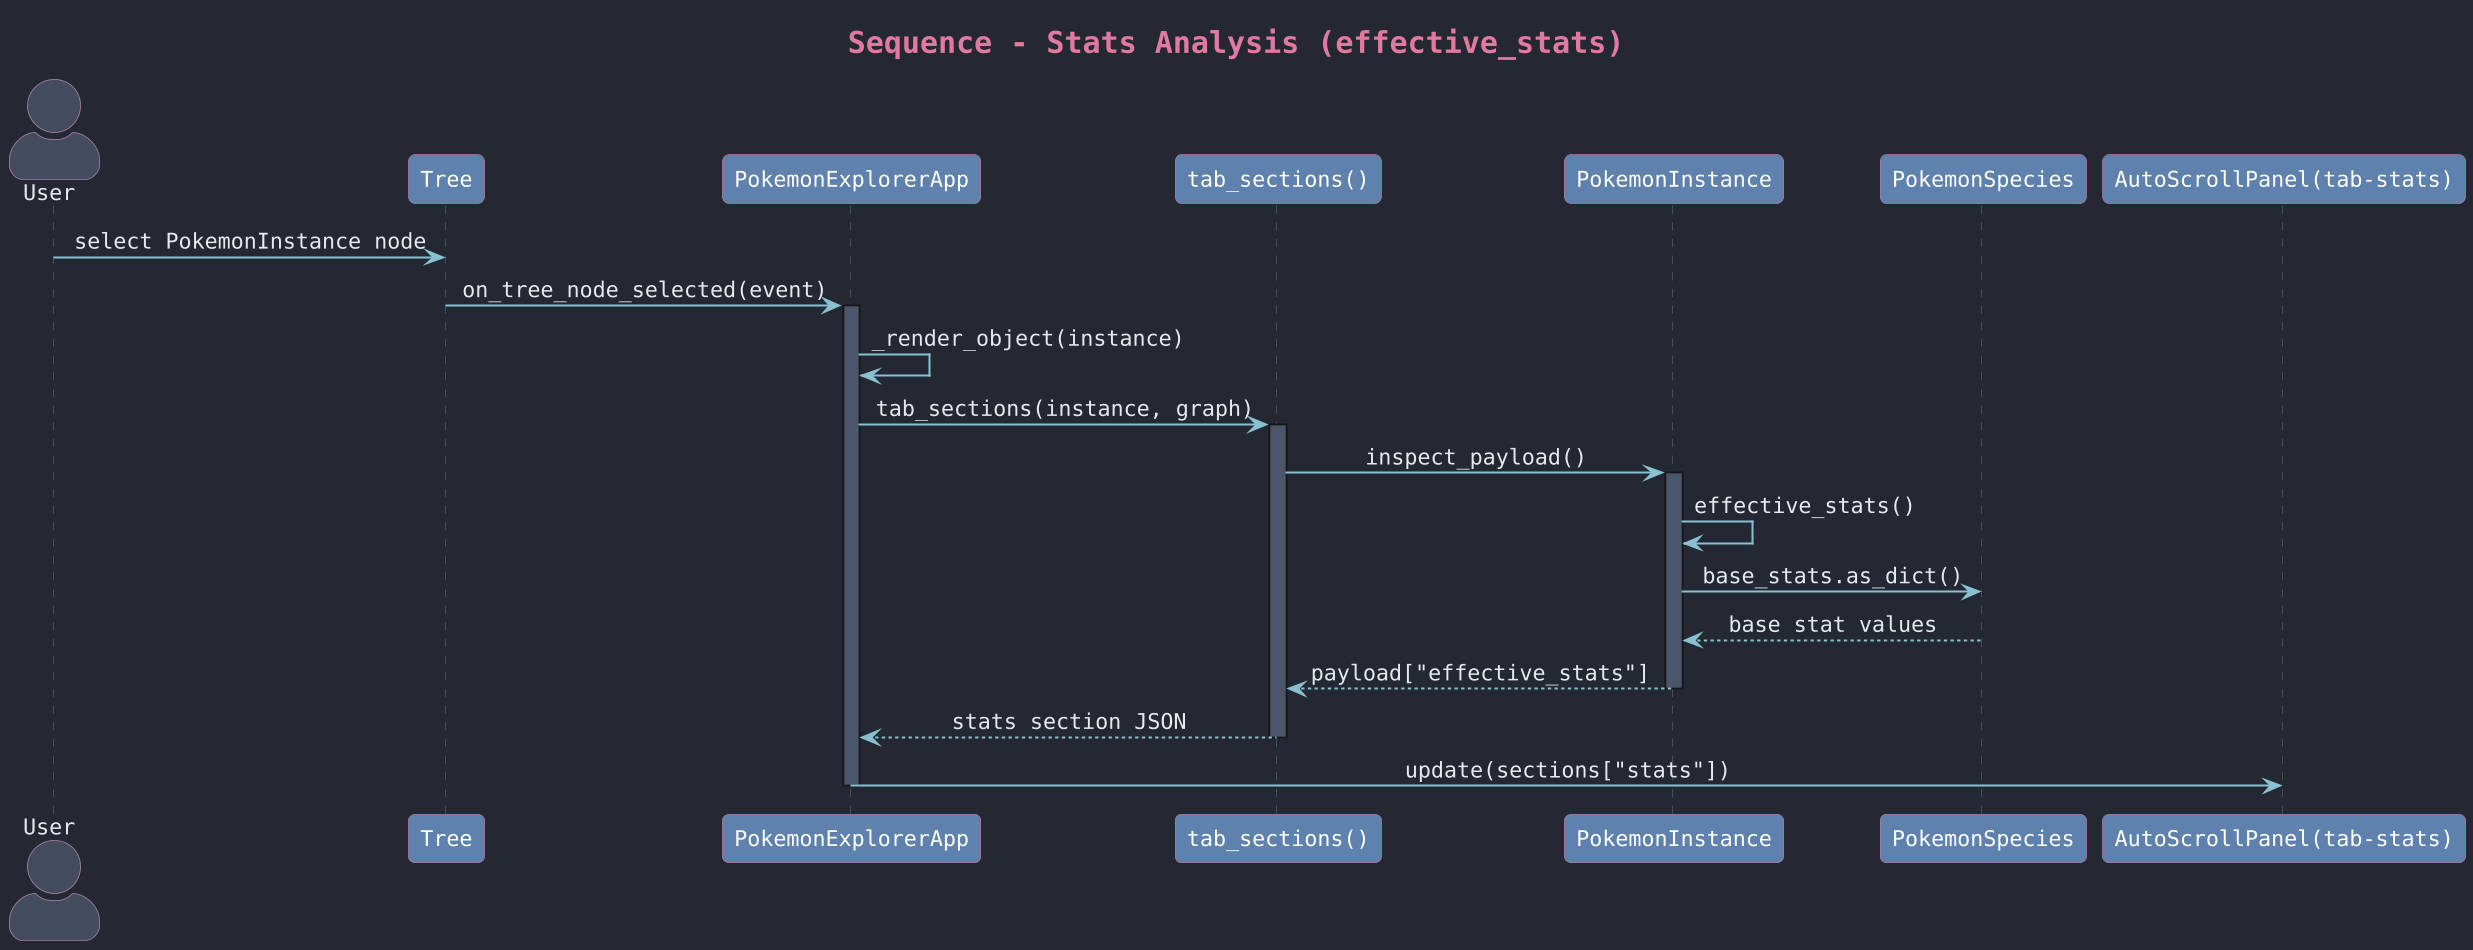
\includegraphics[width=\textwidth,keepaspectratio]{../docs/uml/sequences/images/seq_7_stats_analysis.png}
\end{center}
\textit{Sequence 7: stats analysis (zoom recommended).}

\end{document}
